\chapter{Dynamics of Ion Flux}

\section{Concentrations}
\label{sec:concentrations}

In previous chapter, we use the concept of {\it 'fraction of open channel'}
(Sect.\ref{sec:concentration-example}) to map from a discontinued quantity (i.e.
the number of channel) to a continuous quantity (i.e. fraction in the range 0 to
1). In a generic context of chemical species, an equivalent concept called {\bf
concentration} is used.

Concentration is a way to describe mixture composition, e.g. the
amount of a solvent in a solution. However, this doesn't necessary
liquid ones. 

\subsection{mass (weight/weight) percentage: grams of substance per 100 grams of
sample}
\label{sec:concentration-mass-percentage}

One way is to use mass (weight) percentage (\% w/w)
\begin{equation}
  \label{eq:999}
  \text{c}_{\% w/w} = \frac{m_\text{substance}}{m_\text{solution}} \times 100\%
\end{equation}
In simple case when solution contains only one solvent and one solute,
then $m_\text{solution} = m_\text{solute}+m_\text{solvent}$.  

IMPORTANT: Only weight percentage is the percentage concentration that is always
unambiguous, i.e. does not change with temperature. Unit : (\%). 

\begin{verbatim}
1% w/w means 1 gram of substance per every 100gram of sample
\end{verbatim}

\subsection{mass-volume percentage, volume-volume percentage}

Unlike weight-weight percentage (Sect.\ref{sec:concentration-mass-percentage}),
mass-volume percentage or volume-volume percentage are temperature dependent, so
such quantities are unambiguous.

{\bf Mass-volume (or weight-volume) percentage} (\% w/v) is
\begin{equation}
  \label{eq:1000}
  \text{c}_{\% w/v} = \frac{m_{substance}}{V_{solution}} \times 100\%
\end{equation}
the unit of Volume is [mL], and unit of mass is [g]. So, the overall
unit is in [\% g/mL]. So, it's possible to have solutions of
concentration above 100\% w/v. 



{\bf Volume-volume percentage} (\% v/v) is
\begin{equation}
  \label{eq:1001}
  \text{c}_{\% v/v} = \frac{V_{substance}}{V_{solution}} \times 100\%
\end{equation}
The problem with this usage is that ``volume is only additive for
ideal gas only''. So, the final volume is not a sum of volumes used
when preparing mixture. It means that volume-volume percentage doesn't
sum to 100\%. To convert between concentration types, we need to know
densities of the solution and of both pure solvent and solute. 


\subsection{parts per million/billion: ppm, ppb}

For very low concentration, people often use {\bf ``parts per''}
notation. 

NOTE: \verb!1% w/w! above can be understood as ``1 mass part per
hundred mass parts'', though very rarely used. Instead, these are
often used
\begin{verbatim}
ppm     =  parts per million (10^6)
ppb     =  parts per billion (10^9)
ppt     =  parts per trillion (10^12)
ppq     =  parts per quadrillion (10^15)
\end{verbatim}

``ppq'' is rather a theoretical construct than a useful thing. It can
also use volume by volume, rather than mass by mass. 

Example: 1mL of \ce{SF6}(g) added to 1000L of hydrogen \ce{H2}(g) is 1ppm
vol/vol, but 73 ppm mass/mass. Another example: 1 atom of lead per $10^6$
beryllium atoms there are 23 ppm of lead mass/mass.

\subsection{molar concentration: M (or mole/(Liter solution)), mM, $\mu$M, nM}
\label{sec:concentration-Molar}

{\bf Molar concentration} (M, mM, $\mu$M, nM) or {\bf molarity} is
\begin{equation}
  \label{eq:1002}
  c_M = \frac{n_{substance}}{V_{solution}}
\end{equation}
with unit is [mole/L] or [Molar] or [M].

NOTE: Some old books use M/500 unit, it means 1 mol per 500 litres of solution
(or M/500 means 0.002 mol/L).

\textcolor{red}{Molar concentration is the most often used concentration unit as
it makes stoichiometric calculations much easier}, which can be measured with
the highest precision and for most analytical applications this is the preferred
way of expressing concentration.

{\it The only drawback is that it's temperature-dependent}, e.g. the volumes
increase when the temperature increase and molar concentration goes down. 
To avoid temperature dependency, we can use {\bf molarity}
(Sect.\ref{sec:concentration-molarity}).

\subsection{-- molarity (mole/kg)}
\label{sec:concentration-molarity}

Unlike {\it molar concentration} concept (Sect.\ref{sec:concentration-Molar});
{\bf molarity} is temperature independent.
\begin{equation}
  \label{eq:1003}
  c_m = \frac{n_{substance}}{m_{solvent}}
\end{equation}
is expressed in [mole/kg] units. 

NOTE: It's rarely used in analytical chemistry, molality is often used in {\bf
physical chemistry}, especially when dealing with substance properties over a
wide range of temperature, or properties change with both temperature and
mixture composition.

\subsection{-- normality}
\label{sec:concentration-normality}

{\bf Normality} (similar to molarity, but use equivalent, not moles) has the
units number of [equivalents per Liter]. 

So, the same solution can have different normalities for different types of
reactions. So, it's \textcolor{red}{reaction-dependent}. E.g.: 1M sulfuric acid
solution is 2N for acid/base reactions, and 1N in the reaction of barium sulfate
precipitation.

\begin{framed}
  Molar mass of the substance
  \begin{equation}
    \label{eq:1005}
    n_\text{substance} = \frac{m_\text{substance}}{m_M}
  \end{equation}
with $n_\text{substance}$ is the number of moles. 
\end{framed}

\subsection{Molar fraction}
\label{sec:concentration-molar-fraction}

{\bf Molar fraction} is the number of moles of a substance divided by
the total number of moles of all substances. So the range of a value for molar
fraction is from 0 to 1 and {\bf unitless}. The quantity is temperature
independent.

Conversion:
\begin{enumerate}
\item from weight percentage to molality 
  \begin{equation}
    \label{eq:1004}
    c_m = \frac{1000\times c_{\% w/v/}}{m_M(100-c_{\% w/w})}
  \end{equation}
the factor 1000 is necessary as molality is in [mole/kg] while all
masses are in grams (gr). 
\end{enumerate}

\subsection{protein concentration (mg/ml)}
\label{sec:concentration-protein}


In biochemistry, protein concentration is measured in mg/ml, and is measured
using Bradford method (Coomassie Blue reagent; Pierce Chemical
Co., Rockford, IL) with bovine serum albumin (Sigma Chemical, Co.) as standard. 

Reference:
\begin{itemize}
\item \url{http://www.chembuddy.com/?left=concentration&right=concentration-follies}.  
\end{itemize}


\subsection{Faraday constant}
\label{sec:Faraday-constant}

The particles are often electric charges, whose unit is
Coulomb (C). Definition:
\begin{itemize}
\item {\it 1 Coulomb is the amount of charge that must pass through an
    electrolytic cell in order to deposit $1.1180\times 10^3$g of silver
    from a solution of silver nitrate}, or

\item 1 Coulomb is the amount of charge on $6.242\times 10^{18}$
  electrons. 
\end{itemize}
So, the charges on one mole of electrons (which is Avogadro number
$N_A=6.023\times 10^{23}$ of electrons) is
\begin{equation}
  \label{eq:1343}
  \frac{N_A}{6.242\times 10^{18}} = 9.649\times 10^4 (\C/\text{mol. electrons})
\end{equation}
This quantity is known as {\bf Faraday constant}
\begin{equation}
  \label{eq:1344}
  1\text{ Faraday } = 9.649\times 10^4 \;\;(\C/\text{mol. electrons})
\end{equation}
Faraday's constant converts quantity of moles to quantity of charge for a
univalent ion, i.e. $z=1$. 

\section{Flux $J$}
\label{sec:fluxes}

A flux describes the rate of a reaction, i.e. the speed of reaction
(Sect.\ref{sec:speed-reaction}). In the previous example, we studied the simple
example of the rate of switching between open and close of a cluster of $N$ ion
channels (Sect.\ref{sec:flux-example}).

In chemical reactions, the fraction of 'open' channel in that example is
replaced by the 'concentration' of a given species
(Sect.\ref{sec:concentration}), and the {\bf chemical flux} is used to study the
rate of chemical reactions (Sect.\ref{sec:chemical-flux}).


% \subsection{Current density}
% 
% To avoid the variation between cells, all quantities are determined
% based on a unit of membrane area, except the voltage. The information
% is given in Table~\ref{tab:terminology_2}.
% 
% \begin{table}[hbt]
%   \begin{center}
%     \caption{Ionic currents}
%     \begin{tabular}{p{2cm}r} 
%       \hline
%       notation & description \\ 
%       \hline\hline
%       $I_i$ & ionic current through plasma membrane ($I_{\ce{Na}},
%       I_{\ce{K}}$) \\
%       & ...$I_i = g_i(V_m-E_i) $ \\
%       $I_{app}$ & applied step current (rectangular pulse) (mA/cm$^2$)\\
%       $I_m=\frac{I_0}{A}$ & the current density per unit area (mA.cm$^{-2}$) \\
%       $i_m$ & the current density per unit length (mA/cm) \\
%       $I_\dhpr, I_\LCC$,  $I_\Ca$       & the calcium current via DHPR (L-type channels) \\
%       $I_\ryr$ & the current of calcium released via RyR from JSR \\
%       $I_\Na$ & the current of sodium \\
%       $I_\NaCa$ & the current via Na/Ca exchanger \\
%       $I_\K$ & the current via potassium channel \\
%     \end{tabular}
%   \end{center}
%   \label{tab:Current}
% \end{table}
% 
% With different types of ions, there are respectively different ionic
% currents, Table \ref{tab:Current}. Typically, all currents are indeed
% ``current density'', i.e. in unit [Ampere/unit square], e.g. mA/cm$^2$.

\subsection{Atomic vibrations: thermal energy}
\label{sec:thermal-energy-distribution}
\label{sec:atomic-electronic-energy}
\label{sec:electronic-energy}

Heat causes atoms to vibrate.  The vibration amplitude increases with
temperature.

When vibration are sufficient large to break the bonds, a material is
disruptly transformed from one state to another, e.g. from solid to liquid.

\begin{itemize}
  \item vibration frequency: $10^{13}$ Hz
  
  \item heat provides the atoms an amount of energy, called
  atomic/electronic energy.
  
  Heat causes atomic vibration which generate an amount of energy, called
  atomic/electronic energy.
  
  The average atomic/electronic energy due to thermal excitation is of order of
  $k_B T$, i.e. $E_\text{average} \sim k_BT$ (with $k_B$ = Boltzmann constant,
  and $T$ = temperature in absolute degree Kelvin).

NOTE: $k_BT = 0.026$ (eV) for room temperature.
  
The distribution of such energy around the mean follow the Boltzmann
distribution function (Sect.\ref{sec:Boltzmann-equation})

\begin{equation}
P(E) = \exp\left( -E/(k_BT)\right)
 \end{equation}
$k_B = 1.38 \times 10^{-23}	$(J/K) = $8.62\times 10^5 $ (eV/K).  
  
  
\end{itemize}


\subsection{Atomic diffusion: vacancy diffusion (interdiffusion and
self-diffusion)}

Diffusion is material transport by atomic motion from one lattice site to
another. To move from lattice site to lattice site, atoms need energy to break
bonds with neighbors, and to cause the necessary lattice distortions during
motion from site to another. This energy comes from atomic vibration as
mentioned above.

This type of diffusion, i.e. vacancy diffusion, depends on the presence of
vacancies and therefore increases with the vacancy concentration as the
temperature increases.  Motion of vacancies in one direction is equivalent to
motion of atoms in the opposite direction.

Interdiffusion occurs in response to a concentration gradient (more rigorously,
to a gradient in chemical potential).

\begin{figure}[hbtp]
  \centerline{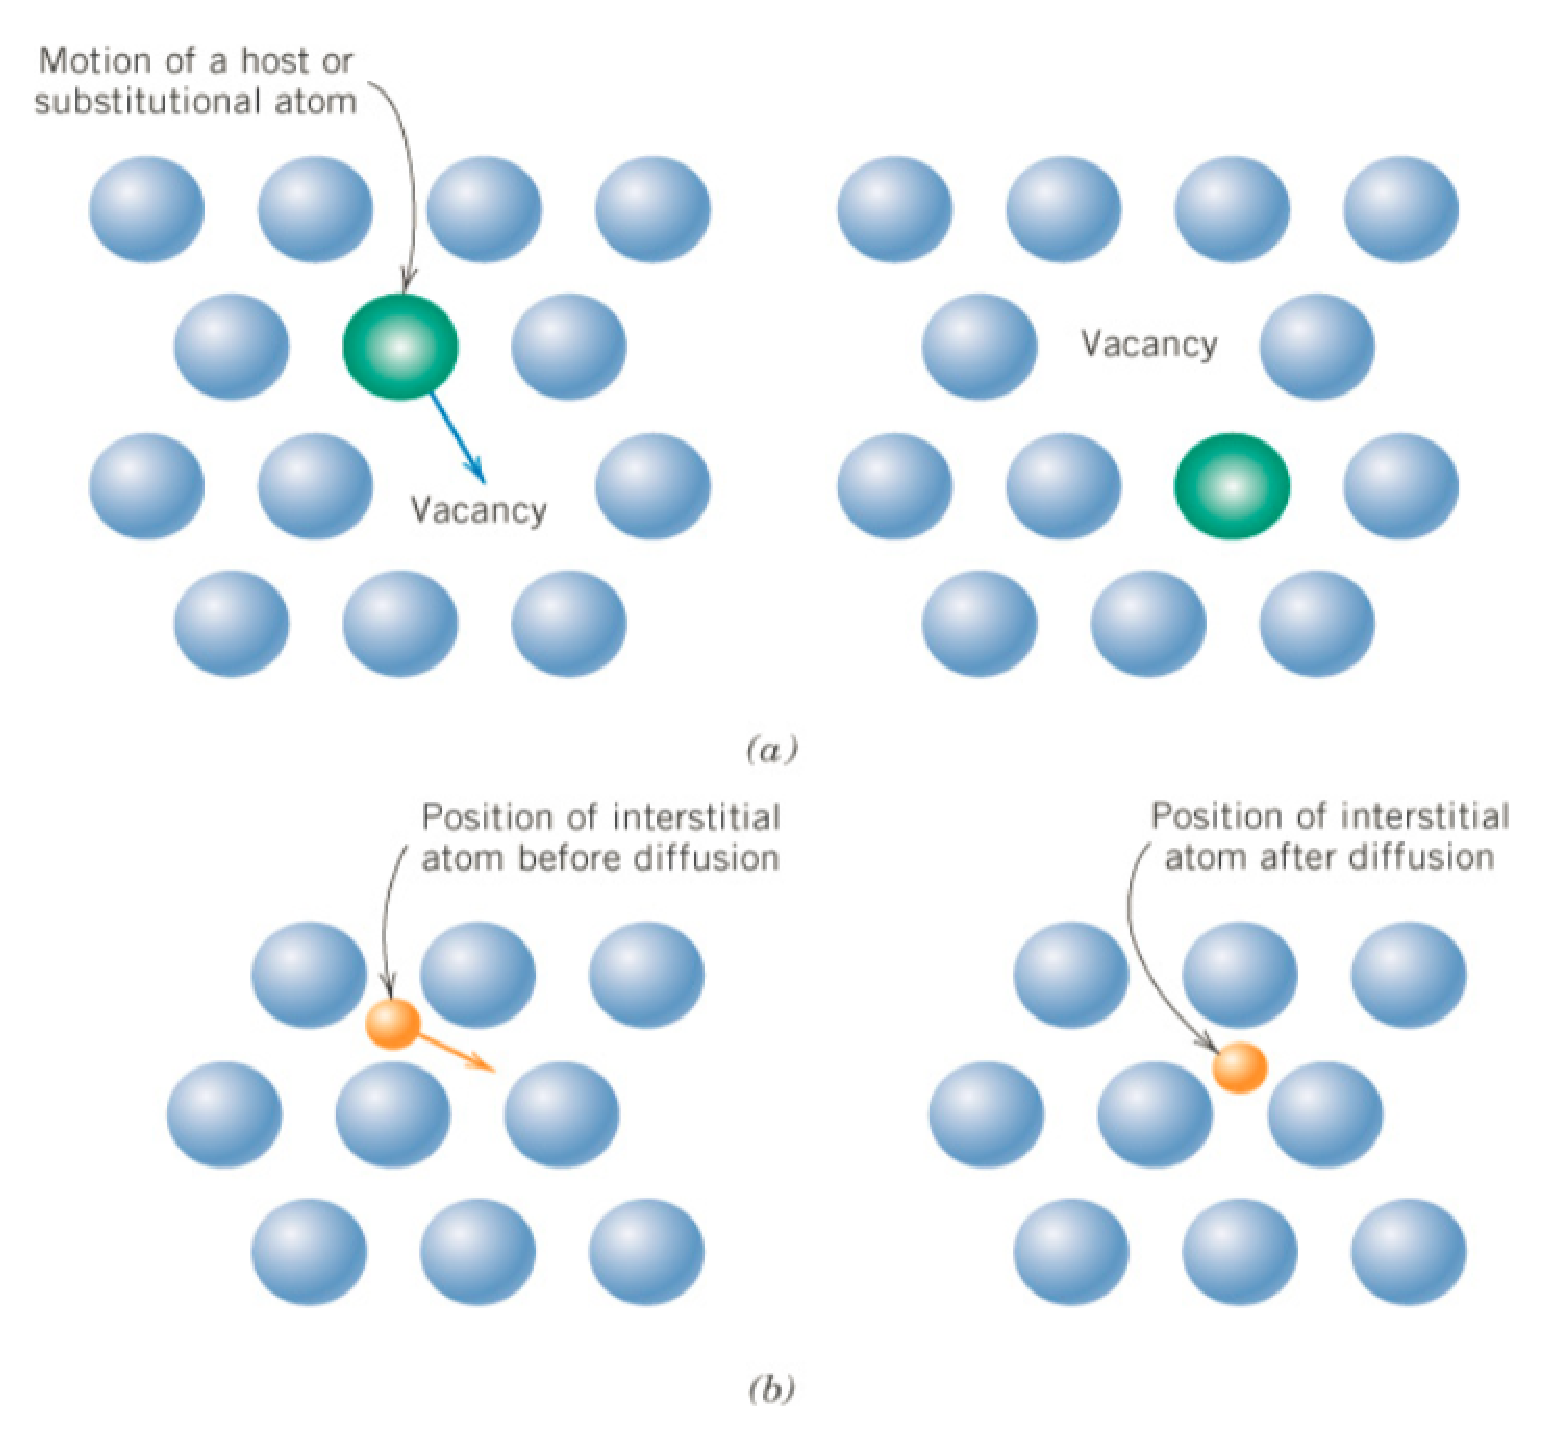
\includegraphics[height=5cm,
    angle=0]{./images/motion.eps}}
\caption{(A) vacancy diffusion; (B) interstitial diffusion}
\label{fig:motion}
\end{figure}

\subsection{Atomic diffusion: interstitial diffusion (interdiffusion only)}

Interstitial diffusion (depends on temperature).  This is generally faster than
vacancy diffusion because there are many more interstitial sites than vacancy
sites to jump to.

\subsection{Probability of energy jump}


\begin{equation}
R_j = R_0 \exp \left( - \frac{E_m}{k_BT} \right)
\end{equation}



\subsection{Diffusion flux (J)}

Diffusion is process which is NOT due to the action of a force , but a result of
the random movements of atoms ( statistical problem).

The flux of diffusing atoms, J, is used to quantify how fast diffusion occurs. 
The flux is defined as either in 
\begin{enumerate}
  \item  number of atoms diffusing through unit area and
per unit time, i.e. atoms/(m$^2$.second).

  \item mass flux: mass of atoms diffusing through
unit area per unit time, (e.g., kg/(m$^2$.second))
\end{enumerate}

\begin{equation}
J = \frac{M}{A.t} = \frac{\text{mass (or atoms or
moles)}}{\text{(cross-sectional area) x time}}
\end{equation}
unit of J (g/(cm$^2$.sec)) if M is mass (g).

In differential form, the instantaneous flux $J$ is
\begin{equation}
J(t) = \frac{1}{A} \frac{\partial M}{\partial t}
\end{equation}

\subsection{Steady-state diffusion: Fick's first law}

In 1D, at steady state of an isothermal, isobaric system, the diffusion along
the direction $x$ is proportional to the concentration gradient.
\begin{equation}
J = - D \frac{dC}{dx}
\end{equation}
As the slope of the change from high to low concentration 
\begin{equation*}
dC/dx = \frac{c_\text{dest}-c_\text{source}}{dx} < 0
\end{equation*}
as $c_\text{dest}=c_\text{low}$ < $c_\text{source}=c_\text{high}$, the minus sign indicate the flux
get positive value and flows in the direction down the concentration gradient. 

$D$ is the diffusion coefficient (Sect.\ref{sec:diffusion-coefficient}), and is
typically chosen as a constant as a given temperature.

\subsection{Diffusion coefficient: Diffusion constant}
\label{sec:diffusion-constant}
\label{sec:diffusion-coefficient}

Diffusion coefficient is the measure of mobility of diffusing species.
At steady-state, the diffusion coefficient is considered a constant value at a
given temperature.
\begin{equation}
D = D_0 \exp \left( - \frac{Q_d}{RT} \right)
\end{equation}
with 
\begin{itemize}
  \item  $D_0 =$ temperature-independent pre-exponential (m$^2$/sec);

\begin{equation}
D_0 = \frac{k_BT}{h}
\end{equation}  
with $h = $ Planck's constant ($6.6 \times 10^{-34}$ J/sec), and $k_B = $
  
  \item $Q_d$ = activation energy for diffusion (J/mole, or eV/atom)
  
  \item $R = $ universal gas constant ()
  
  \item $T = $ temperature (K)
\end{itemize}
If we take the log on both sides
\def\ln{{\text{ln}}}
\begin{equation}
\ln D = \ln D_0 - \frac{Q_d}{R} \left( \frac{1}{T} \right)
\end{equation}
or
\def\log{{\text{log}}}
\begin{equation}
\log D = \log D_0 -\frac{Q_d}{2.3 R} \left( \frac{1}{T} \right)
\end{equation}

\subsection{Nonsteady-state diffusion: Fick's second law}


In most real situations the concentration profile and the the diffusion flux and
the concentrations change with time, i.e. the concentration gradient are
changing with time, Fig.\ref{fig:diffusion-in-time-space}.

\begin{equation}
\frac{\partial C}{\partial t} = \frac{\partial}{\partial t}\left( D
\frac{\partial C}{\partial x} \right) = D \frac{\partial^2 C}{\partial x^2}
\end{equation}

So the time-varying diffusion follows the so-called Fick's second law.

\begin{figure}[hbtp]
  \centerline{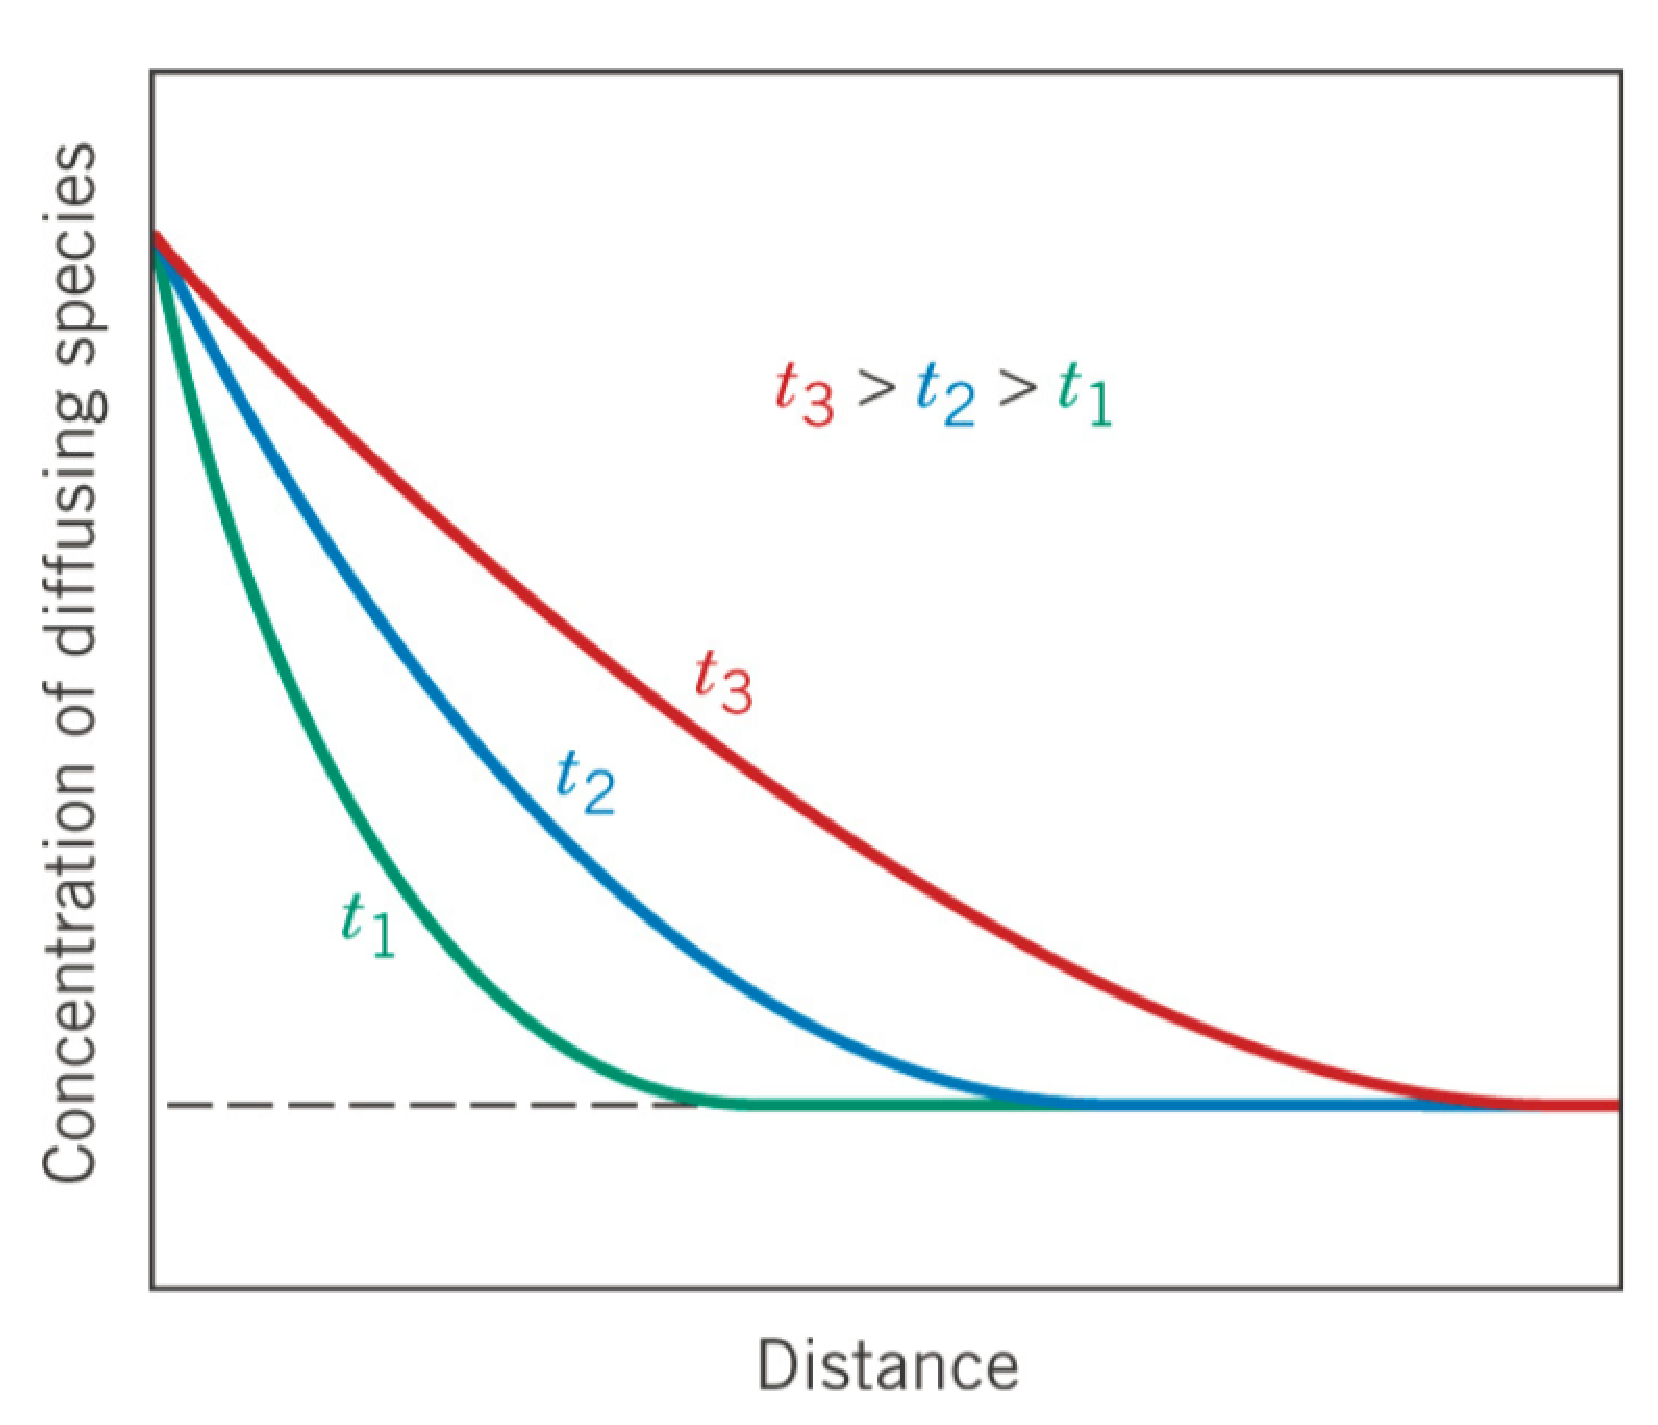
\includegraphics[height=5cm,
    angle=0]{./images/diffusion-in-time-space.eps}}
\caption{Diffusion in time and space}
\label{fig:diffusion-in-time-space}
\end{figure}


Diffusion constant $D$ (distance$^2$/time) is a quantity that tell how fast a
species is translocated from one place to another based on Fickian Law
(deterministic). For a given distance $x$ (distance), the time for movement
is defined as
\begin{equation}
t = \frac{x^2}{2*D}
\end{equation}
The time-constant for this transfer is known as the reciprocal of the time,
$\tau$ (sec$^{-1}$)
\begin{equation}
\tau = \frac{1}{t}
\end{equation}

\begin{framed}
  A connection between ionic mobility $u$ and diffusion constant $D$
  is
  \begin{equation}
    \label{eq:1227}
    D = \frac{u.R.T}{|z|F}
  \end{equation}
with T = absolute temperature [K], R = Faraday constant [J/(mol.K)]
\end{framed}

\section{Chemical flux: Fluxes in aqueous media}
\label{sec:chemical-flux}

For (transmembrane) flux of currents via (selective pores) ion channels, let's
check Sect.\ref{sec:equat-ionic-curr}. In this section, we discuss flux across
two compartments
\ref{sec:flux-example}
\ref{sec:fluxes}

In transport phenomena, a flux is defined as the amount of a substance
that flows through a unit area (or unit volume) per a unit of
time. Generally, the amount is in term of density (e.g. mass per unit
volume or mass per unit surface area), so a flux is a vector.  In
chemical diffusion, the unit of flux
\begin{itemize}
\item can be (mol.cm$^{-2}$.s$^{-1}$) 
\item  or (mol.cm$^{-3}$.s$^{-1}$)

\item or (mol.L.s$^{-1}$) or ($\mu$M/sec).
\end{itemize}
We typically use \verb!cm! rather than metre in chemical diffusion.

There are 4 physical laws that dictates the movement of ions
\begin{enumerate}
\item drift movement under electric field (Sect.~\ref{sec:drift-ions})
\item diffusion of ions under concentration
gradient (Sect.~\ref{sec:ionic-diffusion})
\item the relationship between the two above processes, i.e. the
  diffusion coefficient $D_c$ and the drift mobility $\mu$
  (Sect.~\ref{sec:einstein-relation})
\item the basic principle of separation of charges in biological systems, e.g.
if there is any barrier such as the plasma membrane that separate the two spaces
\end{enumerate}
These laws lead to fundamental equations in computational cell
biology: Nernst-Planck, Nernst, Goldman-Hodgkin-Katz equations, and
Donnan equilibrium equation.

\subsection{Molar flux: Nernst-Planck equation}
\label{sec:flux-molar-flux}
\label{sec:Nernst-Planck-equation}

\textcolor{red}{Effect 1}: The molar flux for diffusive properties in terms of
the diffusion coefficient ($D_s$) and the local concentration of the property
($c_s$). This is Fick's law (Sect.\ref{sec:fickian-diffusion}).

\begin{equation}
M'_s = -D_s \frac{dc_s}{dx}
\end{equation}

\textcolor{red}{Effect 2}: The molar flux of solute due to electrophoretic
effects is defined in terms of the concentration of s (i.e. $c_s$), the
electrical mobility ($u_s$ - the velocity of S in the fluid), and the local
potential ($\Psi$).

\begin{equation}
M'_s = - u_s c_s \frac{d\Psi}{dx} 
\end{equation}


The two affects above are fundamentally additive, i.e.

\begin{equation}
M_s = -D_s \frac{dc_s}{dx} - u_s c_s \frac{d\Psi}{dx}
\end{equation}
This is known as {\bf Nernst-Planck equation} (after Nernst 1888,1889; Planck,
1890). It extends Fick's law for the case where the diffusing particles are also
moved with respect to the fluid by electrostatic forces.
\begin{equation}
\begin{split} 
\frac{\partial c_s}{\partial t} &= -\nabla(J) \\
J &= - \left[ D \nabla c_s - u c_s + \frac{Dz_s e}{k_BT} c_s (\nabla \Psi +
\frac{\partial A}{\partial t}) \right] 
\end{split}
\end{equation}
Its dimension depend on those used to express the ionic concentration an
velocity. NORMALLY: The unit is mol/(cm$^2$.c).

SUMMARY: The total ionic flux for the \verb!k!-th ion type, $\bar{j}_k$, is
given by the sum of ionic fluxed due to (1) diffusion (D), and (2) electric
field (e).
Using {\bf Einstein relationship}
\begin{equation}
\bar{j}_k = \bar{j}_{k,D} + \bar{k}_{k,e} = -D_k \left( \nabla c_k +
\frac{c_k z_k F}{RT} \nabla \Phi \right)
\end{equation}

\begin{mdframed}
Ion flows from one place to another in an aqueous media can be the result from
two driving forces: from an electric field force
(Sect.\ref{sec:flow-by-electric-field-force}) and those resulting from a
diffusional force (Sect.\ref{sec:flow-by-diffusional-force}). For the flow of
ions across a barrier, such as plama membrane, read
Sect.\ref{sec:equat-ionic-curr}.

The {\bf Nernst-Planck equation} describes the flux of an ion (charged
chemical species) in a fluid environment under the affect of diffusion and
electric field.
\begin{equation}
  \label{eq:1228}
    \overrightarrow{j} = \overrightarrow{j_D} + \overrightarrow{j_e} =
    -D (\nabla c + \frac{c.z.F}{R.T}\Delta \Phi) 
\end{equation}
with $\overrightarrow{j}$ = ionic flux [mol/(cm$^2$.sec)]. 
\end{mdframed}

However, what we care about is the current across the membrane, not the molar
flux. It is discussed in Sect.\ref{sec:ionic-flow}.


\subsection{Nerns-Einstein relationship}
\label{sec:Einstein-relationship}

Nernst-Einstein relationship defines 
\begin{equation}
D_s = \frac{u_s RT}{z_s F}
\end{equation}
with $z_s$ is the valence of S.


\subsection{Ionic flows}
\label{sec:ionic-flow}

In order to get from the molar flux (Sect.\ref{sec:flux-molar-flux}) to the
current we need only multiply by the valence and Faraday's constant
\begin{equation}
I_s = z_s.F.M_s
\end{equation}
\ref{sec:nernst-equation}
We can easily convert the ionic flux to the electric current density $I$ by
multiplying the ionic flux by $zF$ (i.e. the number of charges carried
by each mole).

The ionic flux $\bar{j}_k$ can be converted to an electric current density
$I$ by multiplying the former by \verb!z_k.F!
\begin{equation}
I_k = \bar{j}_k \times z.F = -D_k z_k F \left( \nabla c_k +
\frac{c_k z_k F}{RT} \nabla \Phi \right)
\end{equation}
The unit of electric current density $J_{k}$ is [C/(cm$^2$.s)] = [A/cm$^2$].

The equivalent form is
\begin{equation}
I_k = - \left(  \mu_k R T \frac{z_k}{|z_k|} \nabla c_k + u_k c_k
|z_k| F. \nabla \Phi \right)
\end{equation}
\url{http://www.bem.fi/book/03/03.htm}

\begin{mdframed}
\begin{equation}
  \label{eq:1242}
  \begin{split}
    I &= -DzF (\nabla c + \frac{c.z.F}{R.T}\Delta \Phi) \\
     &= - \left(u.R.T.\frac{z}{|z|}\nabla c + u.c.|z|F\nabla\Phi\right)
  \end{split}
\end{equation}
with $I$ = electric current density [C/(sec.cm$^2$)] = [A/cm$^2$].
\end{mdframed}

By integrating the Nernst-Planck equation across the cell membrane -
the center of the membrane is taken as the origin of coordinates for a membrane
of thickness $h$ - for a steady-state and arbitrary potential profile, the
diffusive flux across the cell membrane is (Jacquez, Schultz, 1974)
\begin{equation}
I_k^d = \frac{-h P_k}{\int_{-h/2}^{h/2}  \exp\left( z_k F \psi(x) /(RT)
\right)dx} 
\left[  c_k^i Z^{z_k}_i \exp\left(\frac{z_k F V}{2 RT} \right) 
      - c_k^o Z^{-z_k}_o \exp\left( -\frac{z_k F V}{2 RT} \right)
\right]
\end{equation}
NOTE:
\begin{enumerate}
  \item $P_k$ = permeability of ion $k$ - Sect.\ref{sec:permeability}
  
  \item $z_k$ = valence of ion $k$
  
  \item $\psi(x)$ = the potential at point $x$ along the membrane
  
  NOTE: $\psi(-h/2)$ = from the outside at $-h/2$;
  $\psi(h/2)$ = from the inside at $h/2$
  
  \item $c_k^i, c_k^o$ = the concentration (activity) of ion $k$ at
  intracellular and outer-side of membrane, respectively.
  
  \item $Z$ factor is defined as 
  
\begin{equation}
Z_i = \exp (F V_i /(RT)) \qquad;
Z_o = \exp (F V_o / (RT)) 
\end{equation}
with $V_i = \psi_i - \psi(h/2)$; and $V_o = \psi(-h/2) - \psi_o$ - which are
potential differences between inner and outer bulk phases with the adjacent
membrane surfaces.

NOTE: The transmembrane potential $\Vm = \psi_i - \psi_o = V_i + V + V_o$


\end{enumerate}



\subsection{- caused by electric field force}
\label{sec:flow-by-electric-field-force}
\label{sec:electric-field}

We consider two points: O (with reference potential $\Phi_O$) and P (with
potential $\Phi_P$).  So, the work required to move one unit charge 
is
\begin{equation}
\label{eq:work-move-1-molecule-ion}
W_e = (\Phi_P - \Phi_O)
\end{equation}

Whenever a force exerts on a unit charge, an electric field is defined, in the
opposite direction of the translocation. The {\bf electric field} is defined as
{\it the force that exerts on a unit charge}.

The work $W_e$ required to move Q quantity of charge from
point O to point P is
\begin{equation}
W_e = Q (\Phi_P - \Phi_O)
\end{equation}
with $W_e$ [Joules, J], $\Phi$ [Volt], Q [Coulomb, C]). 

\begin{mdframed}
Instead of using Coulomb, the quantity of ions in electrophysiology is often
used as {\it moles}. Suppose the valence of an ion is $z$ and the change on one
mole of electrons is $F$ (Faraday constant), then the work required to move one
mole of an ion (i.e. an $N_A$ number of molecules of
that ion) of valence $z$ [unitless] from point O to point P is
\begin{equation}
W_e = zF (\Phi_P - \Phi_O)
\end{equation}
NOTE: for $\Ca$ ion, $z_\Ca = 2$.

\end{mdframed}

The work required to move a unit positive charge (i.e. $Q=1$) from O to P (of
distance $ds$) against the electric field $\vec{E}$ is defined as
\begin{equation}
dW = - \vec{E} \cdot \vec{ds}
\end{equation}
with $\vec{ds}$ is the vector of displacement.


Combined with eq.\ref{eq:work-move-1-molecule-ion}, we have
\begin{equation}
\Phi_P - \Phi_O = - \vec{E} \cdot \vec{ds}
\end{equation}

Applying Taylor series expansionof the scalar field $\Phi$ around the point O
along the path $s$
\begin{equation}
\Phi_P = \Phi_O + \frac{d\Phi}{ds} ds + \ldots
\end{equation}
The second term is known as {\it directional derivative of $\Phi$ in the
direction $s$} and by vector-analytic properties of the gradient is given by
$\nabla \Phi \cdot \vec{ds}$. 

If P is very close to O, the remaining higher terms may be neglected. So, we
have $\Phi_P - \Phi_O = \nabla \Phi \cdot \vec{ds}$.


\subsection{- caused by diffusional force}
\label{sec:flow-by-diffusional-force}

If the ionic concentration is not uniform between adjacent compartments, this
leads to a passive redistribution of ionic concentration, which can be described
using {\bf Fickian diffusion} formula (Sect.\ref{sec:ficks-law-diffusion})
\begin{equation}
  \label{eq:1226}
  \overrightarrow{j_D} = -D\nabla c
\end{equation}
with D = diffusion constant [cm$^2$/sec] (Sect.\ref{sec:diffusion-constant}), c
= ionic concentration [mol/cm$^3$] (or Molar=mole/litre), $\overrightarrow{j_D}$
[mol/(cm$^2$.sec)].


\subsection{-- ((((()))))}
In a metabolism process, the product C of one reaction can be the input (i.e.
the reactant) of another one. Hence, the concentration of C, i.e. [C], can
change due to either the consumption of C or the production of C.
Sect.\ref{sec:concentration} describes how a concentration is defined.

\begin{equation}
  \label{eq:135}
  \begin{split}
    \ce{A + B <=> C} \\
    \ce{C + D -> E}
  \end{split}
\end{equation}

The amount of C (in moles) that create/consumed in a unit volume per
unit of time is called the
{\bf chemical flux}\footnote{\url{http://en.wikipedia.org/wiki/Flux}}
of species C, denoted by $J$. 

The equation is given
\begin{equation}
  \label{eq:85}
  J = [C]k
\end{equation}
with $[C]$ is the concentration of the product C
[mol.m$^{-3}$.s$^{-1}$], $k$ is the reaction rate.

{\bf NOTE}: Flux (from Latin: fluxxus - flow)
{\it indicates the amount of flow go through a unit of surface (area)
  per unit time}.
There are different context for using flux, here, we talks about
{\bf chemical flux}, denoted by $J_{chem}$ [mol.m$^{-3}$.s$^{-1}$].

If we can call the amount of C produced in a unit time is $J_{in}$ and
the amount of C consumed in a unit time [s] is $J_{out}$, then the
change in concentration (in the direction of adding) of C in a unit
time [s] is
\begin{equation}
  \frac{d[C]}{dt}=J_{in} - J_{out}
\end{equation}

Let's consider an isobaric, isothermic reaction, i.e. $p=const,
T=const$. Then, based on eq. \eqref{Gibbs} introduced in the previous
chapter, the change in Gibb's free energy of a particular substance is
\begin{equation}
  \label{eq:64}
  dG= -SdT + \mu dN + Vdp = \mu dN
\end{equation}
with $\mu$ is the
{\bf chemical
  potential}\footnote{\url{http://en.wikipedia.org/wiki/Chemical_potential}},
i.e.the potential per mole.


Chemical potential of a component in a solution can be thought of in
many
ways\footnote{\url{http://www.geol.umd.edu/pages/facilities/lmdr/chmpot.htm}}.
In our case, it is defined as the rate at which the extensive internal
energy increase as the number of moles of the component in question
increase.
\begin{equation}
  \label{eq:136}
  \mu = \frac{\partial U}{\partial N_i}|_{S,V,N_{j\neq i}} 
\end{equation}
Its unit is {\it the ``energy'' per mole} [J/mol], $dN$ is the change in
the number of moles for such substance (negative for loss,
positive for gain). Under such condition, the change in the Gibb's
free energy is caused by the change in the number of moles.
% or its variant {\it ``energy'' per mole}

{\bf NOTE}: In general thermodynamics, studied particles don't have to
be only atoms or molecules (i.e. the objects of chemistry). They can
be electrons, holes, or anything else that can be identified and
numbered. The ``chemical potential'' of the electrons, however, is
still a major parameter of the system (to the annoyance of the solid
state physicists - they therefore usually call it ``Fermi
energy'')\footnote{\url{http://www.tf.uni-kiel.de/matwis/amat/def_en/kap_2/advanced/t2_4_1.html}}.



\section{Flux within a single compartment}
\label{sec:flux-within-compartments}

Flux within a single compartment refers to the rate of formation or losing of a
species, i.e. the amount of change over a unit of time, e.g. $J_E = d[E]/dt$.

\section{Flux across compartmental border}
\label{sec:flux-across-compartments}

When spatial dimension is considered, then we need to also estimate the
the flux, i.e. concentration change, due to diffusion from one compartment to
another.


\section{Duffision}
\label{sec:diffusion}

\subsection{Diffusion formula}

Depending on the diffusion, the
formula can be simplified in two ways
\begin{enumerate}
\item isotropic:
  \begin{equation}
    \label{eq:1430}
    \nabla.(D_C\nabla[\Ca]) = D_C(\partial^2[Ca]/\partial r^2 +
    (2/r)\partial[\Ca]/\partial r)
  \end{equation}

\item anisotropic:
  \begin{equation}
    \label{eq:1431}
    \nabla.(D_C\nabla[\Ca]) = D_{Cx}\partial^2[\ca]/\partial x^2 +
    D_{Cy}\partial^2[\ca]/\partial y^2 + D_{Cz}\partial^2[\ca]/\partial z^2 
  \end{equation}
\end{enumerate}


\subsection{How fast of a diffusion: effective diffusion constant}
\label{sec:effective-diffusion-constant}

Under a standard environment ({\it in vitro}), the diffusion of a species is
known as true diffusion. However, under an {\it in vivo} environment, the diffusion can be
slower, due to the viscosity in the media, etc. This diffusion is known as {\bf
effective diffusion constant}. To model kinetics of species inside the cell, we
need to consider using effective diffusion constants, and similarly with
effective volume (to be discussed in the next section).




\section{Currents (movements of ions)}
\label{sec:currents}

Current is the total amount of positive charges (in unit of Coulombs) flowing
across a fixed point in the wire per unit of time
\begin{eqnarray}
  \label{eq:409}
  I = \frac{dQ}{dt}
\end{eqnarray}
with the unit of current is {\bf Ampere} = A = Coulomb/sec = C/sec
(Sect.\ref{sec:current-ampere}).

The current is often calculated using the formula
\begin{equation}
I_s = \bar{g}_S \times \left(  \text{driving forces} \right)
\end{equation}
with the driving force can be
\begin{enumerate}
  \item linear - Sect.\ref{sec:ohms-law}
  
  \item non-linear - Sect.\ref{sec:GHK_current}
\end{enumerate}

\subsection{current in physics}
\label{sec:current-in-physics}

By convention, in physics, current is the direction of the movement of positive
charge (or the opposite sign of the electron movement).

\subsection{current in electrophysiology}
\label{sec:current-in-electropysiology}
\label{sec:ionic-currents}

By convention, in physics, current is the direction of the movement
of positive charge (or the opposite sign of the electron movement). 

However, in electrophysiology, the sign of the (density) current is positive if
the positive charged ion moves from inside to outside of the cell, and vice
versa. This is opposite for negative charged ions, e.g. $\Cl$. For the stimulus
current, if we use

\begin{equation}
  \label{eq:1365}
  \Csc \frac{dV_m}{dt}=-I_\ion + I_\stim
\end{equation}
then $I_\stim$ (from outside to inside) is positive. Otherwise, if we
use
\begin{equation}
  \label{eq:1366}
  \Csc \frac{dV_m}{dt}=-(I_\ion + I_\stim)
\end{equation}
then $I_\stim$ (from outside to inside) is negative. Again, the unit
$\Csc$ is $\mu$F/cm$^2$, and $V_m$ is [mV], while $I_\ion, I_\stim$ is
in $\mu$A/cm$^2$. 

\begin{figure}[hbt]
  \centerline{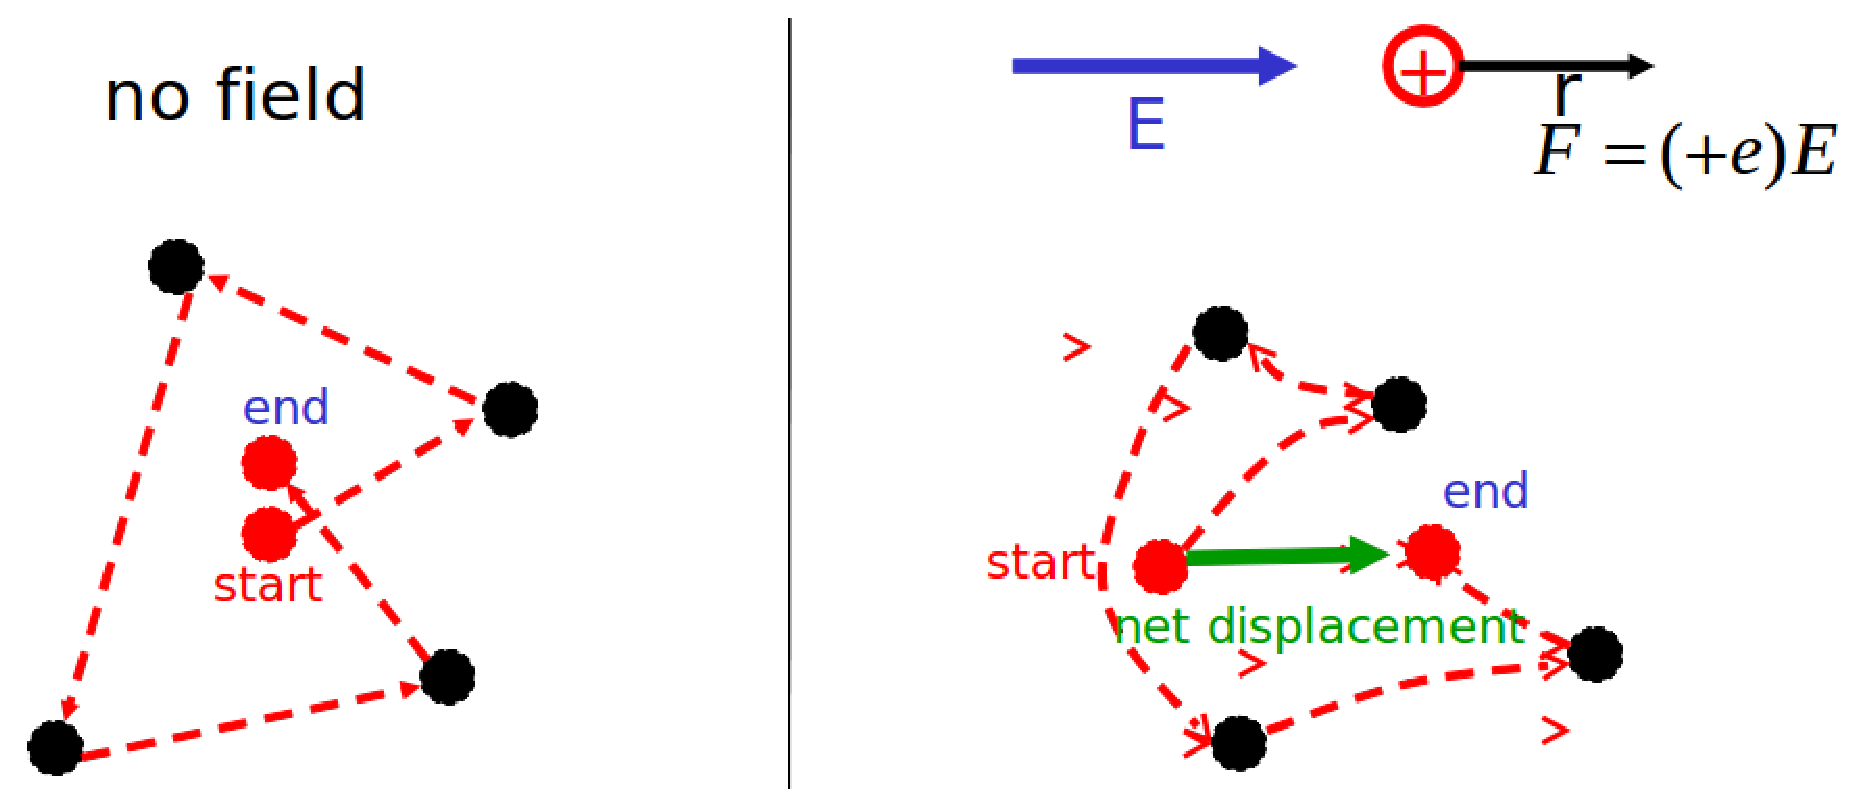
\includegraphics[height=4cm,
    angle=0]{./images/electric_field.eps}}
  \caption{Electric field}
  \label{fig:elec_field}
\end{figure}


At a point in space, using Kirchoff's law (i.e. the law of conservation), the
applied current $I_\app$ is equal to the sum of the membrane current via
capacitor $I_m$ and the ionic current $I_\ion$ (positive if outward),
Fig.~\ref{fig:electric_current}.
\begin{equation}
  \label{eq:689}
  I_\app = I_\ion + I_m + I_{\text{axial}}
\end{equation}
with unit [ampere/unit area]. NOTE: $I_m = \frac{dV_m}{dt}$ 
%So, the transmembrane current $I_m$ is given by
%the sum of the ionic currents and the current flowing into the membrane
% capacity
If we convert to density current, i.e. current per unit surface area, then
\begin{equation}
\Csc \frac{dV_m}{dt} = - \sum j_{ion} + \frac{1}{A} I_\app - j_{\text{axial}}
\end{equation}
with the equation of individual inonic currents $I_{ion}$ can be selected from
Sect.\ref{sec:equat-ionic-curr}.

\begin{enumerate}
  \item current density: nA/$\mum^2$
  \item specific membrane capacitance: $\mu F/\mum^2$
  \item surface area (A) : $\mum^2$
  \item current injection ($I_\app$): nA
\end{enumerate}

If an AP is initiated at all points along the fibre simultaneously, the membrane
potential at all points along the fibre would be the same (or uniform). Then the
axial current $I_{\text{axial}}$ will therefore be zero. 
% This type of response is called a 'membrane' action potential by
% Hodgkin-Huxley, and is rewritten with $I_m=0$ \citep{noble1962mhh}.

Finally, we obtain the widely use formula to model the electrical
property of a cell membrane
  \begin{equation}
    \label{eq:33}
    \Csc \frac{dV_m}{dt} = -\sum_i g_i (V_m-E_i) + \frac{1}{A} I_\app %+
    % I_{\text{axial}}
  \end{equation}
with $\Csc$ in ($\mu$F/cm$^2$), $V_m$ in [mV], $g_i$ in (mS/cm$^2$),
and $I_\app$ in ($\mu$A) and $A$ is surface area. 

\subsection{Current: Ampere}
\label{sec:ampere-current}
\label{sec:current-ampere}
The movement of 1 Coulomb per second is known as the unit of
electrical current, denoted as Ampere (A). It means that 1 (A) = 1
(C/sec), or
\begin{equation}
  \label{eq:1345}
  1 \text{ Faraday } = 9.649\times 10^4 (\text{A.sec})
\end{equation}


\begin{table}[hbt]
  \begin{center}
    \caption{Ionic currents}
    \begin{tabular}{p{2cm}r} 
      \hline
      notation & description \\ 
      \hline\hline
      $I_i$ & ionic current through plasma membrane ($I_{\ce{Na}},
      I_{\ce{K}}$) \\
      & ...$I_i = g_i(V_m-E_i) $ \\
      $I_{app}$ & applied step current (rectangular pulse) (mA/cm$^2$)\\
      $I_m=\frac{I_0}{A}$ & the current density per unit area (mA.cm$^{-2}$) \\
      $i_m$ & the current density per unit length (mA/cm) \\
      $I_\dhpr, I_\LCC$,  $I_\Ca$       & the calcium current via DHPR (L-type channels) \\
      $I_\ryr$ & the current of calcium released via RyR from JSR \\
      $I_\Na$ & the current of sodium \\
      $I_\NaCa$ & the current via Na/Ca exchanger \\
      $I_\K$ & the current via potassium channel \\
    \end{tabular}
  \end{center}
  \label{tab:Current}
\end{table}

With different types of ions, there are respectively different ionic currents,
Table \ref{tab:Current}. Typically, all currents are indeed ``current density''
(Sect.\ref{sec:current-density}), i.e. in unit [Ampere/unit square], e.g.
mA/cm$^2$.


\subsection{Current density}
\label{sec:current-density}

In electrophysiology, to avoid the variance in geometry of the cells, the ionic
current measured in one cell is often converted to {\bf current density},
with unit $\mu$A/cm$^2$, or $\mu$A/$\mu$F. This is useful, under the assumption
that regardless of the cell sizes, shapes, the density is pretty much similar
among the cells. So we can use this to develop models for any cell sizes.

Besides current as density, all quantities are determined based on a unit of
membrane area, except the voltage. The information is given in
Table~\ref{tab:terminology_2}.

The {\bf current density} $\overrightarrow{J}$ and electric field
$\overrightarrow{E}$ are related by
\begin{equation}
  \label{eq:1224}
  \overrightarrow{J} = \sigma \overrightarrow{E} = -\sigma \nabla \Phi
\end{equation}
with $\sigma$ is the conductivity of the medium. If we're interested
in the ions, the flux $j$ of these ions are subject to the electric field
force, and is dependent upon the electric resistance, which in turns
is a function of ionic mobility $u$ of the ionic species. 
\begin{equation}
  \label{eq:1225}
  \overrightarrow{j_e} = u \frac{z}{|z|}c\nabla \Phi
\end{equation}
with $c$ is the ionic concentration [mol/cm$^3$], z = valence
[unitless], u = ionic mobility [cm$^2$/(V.sec)], and
$\overrightarrow{j_e}$ = ionic flux (due to electric field)
[mol/(cm$^2$.sec)]. 


\subsection{Drift of ions}
\label{sec:drift-ions}

Major types of ions in the cells are $\K$, $\Na$, $\Ca$, $\Cl$....  In most part
of the body, the space-charge neutrality is applied
(Sect.~\ref{sec:princ-space-charge}). Yet an important exception is in the
plasma membrane of individual cells. The membrane is selectively permeable to
certain ions under certain condition, thus maintaining a concentration gradient
which results in an electric field across the membrane. Near the plasma
membrane, ions moving is not only affected by diffusion
(Sect.~\ref{sec:ionic-diffusion}) but also under the affect of an electric field
$\mathbf{E}$ which is the result of potential gradient.
\begin{equation}
  \label{eq:1368}
  \mathbf{E} = \frac{\partial V}{\partial l} = \nabla \phi
\end{equation}
with $V$ is the voltage, and $l$ is the length.  This electric field exert a
force $\mathbf{F}=q.\mathbf{E}$ on the particle of charge $q$, causing a {\bf
drift of ions}. It means the ion move randomly, but with a net drift velocity,
i.e. the average motion of the ion, is in parallel to the electric field
$\mathbf{E}$.  This {\bf drift velocity} is dependent upon the material of the
transmitting media, and is in the order of millimeters per second in contrast to
the order of the random speed of the electron themselves (million meters per
second)\footnote{The speed of light is 300 million meters per second}, as shown
in Fig.~\ref{fig:elec_field}.

To tell how well a material can accommodate the movement of electric
charges, we use the concept of {\bf electrical conductivity}, the
symbol is $\kappa$ (or $\sigma$ or $\gamma$), with the unit is
[Siemen/metre] (S.m$^{-1}$) which is the ratio of the current density $j$
(A/m$^2$) to the electric field (V/m).
\begin{equation}
  \label{eq:1367}
  \kappa = \frac{j}{|\mathbf{E}|}
\end{equation}
with $|\mathbf{E}|$ is the magnitude of the electric field. 

The drift velocity is constant, and is the product of the magnitude of
the electric field times a constant called mobility $\mu$.
\begin{equation}
  \label{eq:1369}
  v_\drift = |\mathbf{E}|\times \mu
\end{equation}

The drift flux of ions C moving across the electric field is described
by Ohm's law ({\bf Planck's equation})
\begin{eqnarray}
  \label{eq:407}
  J_\drift = \kappa\mathbf{E} = \mu \frac{z}{|z|} [\text{C}] \nabla \phi
\end{eqnarray}
Units
\begin{itemize}
\item $J_\drift$: molecules/(sec.cm$^2$)
\item $\kappa$ is electrical conductivity (conductivity of the
  material): molecules/(V.sec.cm)
\item $\mathbf{E}=-\frac{\partial V}{\partial x}$ is electric field:
  V/cm
\item  $[\text{C}]$ is the concentration of ions C which
  is in [molecules/cm$^3$].
\item V is electric potential (voltage): V
\item $\mu$: mobility : cm$^2$/(V.sec)
\item z is valence of ion, e.g. +1 for \ce{Na+}, +2 for \ce{Ca^2+} :
  dimensionless
\end{itemize}

The current density can be expressed in terms of free charge density
\begin{eqnarray}
  \label{eq:408}
  j=\eta qv_\drift
\end{eqnarray}
with $\eta$ is free charge density (i.e. number of charge carriers per
unit volume), $v_\drift$ is drift (average) velocity of each charge,
$q$ is the charge of a single charge carrier (ions), $q=z.(+e)$. When
the mobile charges has valence +1 (i.e. contribute one free electron),
then $q=e=1.6\times 10^{-19}$ C.


Thus, the current $I$ is the amount of charge pass through a cross
section area A, given that the wire is modeled a shaded disk of area A
and length L.
\begin{eqnarray}
  \label{eq:411}
  I = j\times A =  \eta qAv_\drift
\end{eqnarray}
\begin{figure}[hbt]
  \centerline{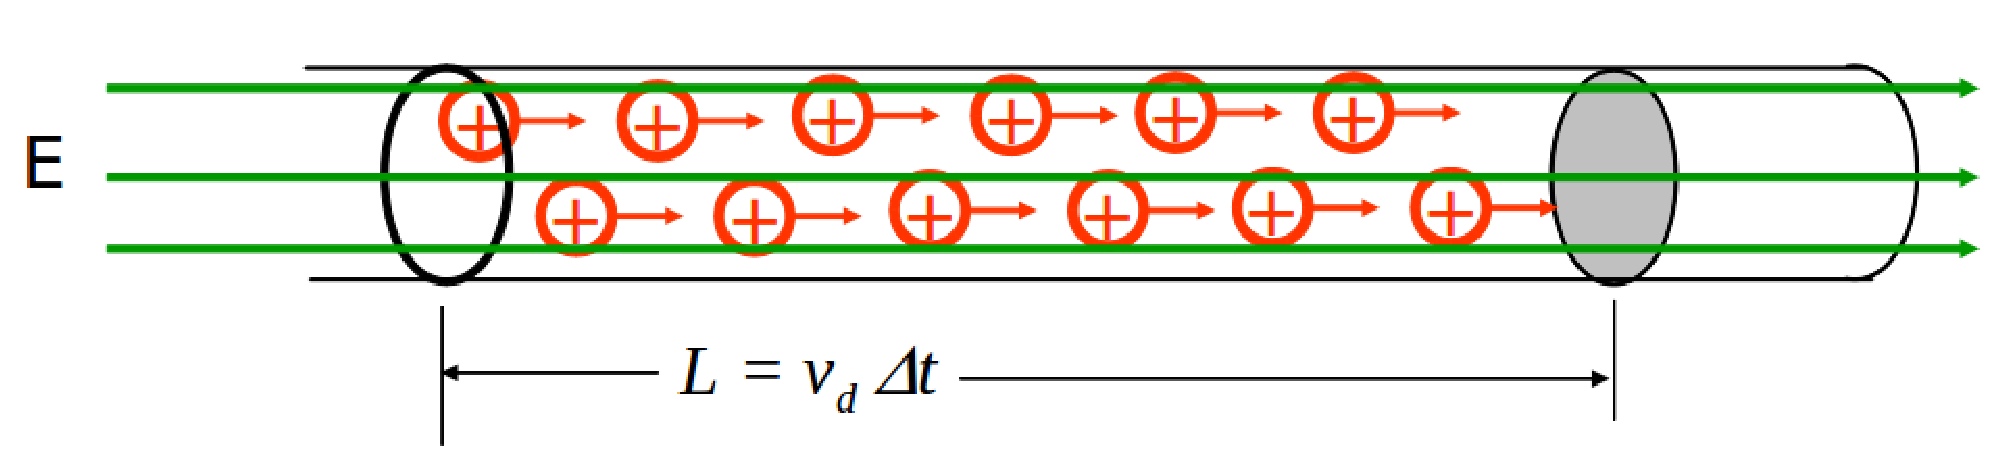
\includegraphics[height=2cm,
    angle=0]{./images/current.eps}}
  \caption{Current}
  \label{fig:current}
\end{figure}

{\bf Quizz}: A copper wire of cross sectional area $A = 3\times
10^{-6}$m$^2$ carries a current of $I=10$A. Find the drift velocity of
the electrons in this wire $v_\drift$. Copper has a density of
$k=8.95$ g/cm$^3$, and atomic weight is
$m_a=63.5$g/mole. Avogadro's number is $Avog.=6.02\times 10^{23}$
atoms. Assume each atom contributes one free electron.

{\it Solution}:  The number of mole per a unit volume is
$\frac{k}{m_a}$. In a single mole, there are Avogadro number of
molecules. Thus, the number of molecules in a unit of volume of the
wire is $\frac{k}{m_a}\times Avog.$. As each molecule (atom)
contribute one free electron, the number of free electron in a unit of
volume is $\eta\times q = \frac{k}{m_a}\times Avog.$. Finally, the
drift velocity is
\begin{eqnarray*}
  v_\drift = \frac{I}{\eta q A} = \frac{10}{\frac{k}{m_a}\times
    Avog. A}
\end{eqnarray*}


\begin{framed}
  $j$ is proportional to the electric field $\mathbf{E}$
  \begin{eqnarray*}
    j= \sigma \mathbf{E}
  \end{eqnarray*}
  while the potential difference $V=\mathbf{E} L$ with $L$ is the length
  of the wire, and $\mathbf{E}$ is the electric field between the two
  ends of the wire. For a uniform wire, we have
  \begin{eqnarray*}
    V = I \times \frac{\rho L }{A}
  \end{eqnarray*}
  with $\rho = \frac{1}{\sigma}$ (unit: $\Omega m$) is the resistivity,
  the quantity
  \begin{eqnarray*}
    R = \rho \frac{L}{A}
  \end{eqnarray*}
  is the resistance (unit: ohm = $\Omega = \frac{Volt}{Amp}$).
\end{framed}

\subsection{Ionic diffusion}
\label{sec:ionic-diffusion}

Ions in a biological system are not uniformly distributed. The
gradient in ion concentration is the main-driving force of the
diffusion of ions in different compartment of the cell. Physical
principles of ion diffusion is decrsibed in this section.

For simplicity, we consider the case when ions moving in a single
dimension, i.e. along x-axis. This is known as the {\bf Fick's first law}
\begin{equation}
  \label{eq:1370}
  J_\diff = -D \frac{\partial[\text{C}]}{\partial t}
\end{equation}
with $J_\diff$ is [molecules/(sec.cm$^2$)], the diffusion coefficient
is (cm$^2$/sec), and $[\text{C}]$ is the concentration of ions C which
is in [molecules/cm$^3$].


\subsection{Einstein relation}
\label{sec:einstein-relation}

Einstein (1905) derived this relationship

\begin{eqnarray}
  \label{eq:412}
  D = \frac{k_BT}{q}\mu = \frac{\mu RT}{|z|F}
\end{eqnarray}
which formally states that diffusion and drift processes in the same
medium are additive.

\subsection{Principle of space-charge neutrality}
\label{sec:princ-space-charge}

\begin{figure}[hbt]
  \centerline{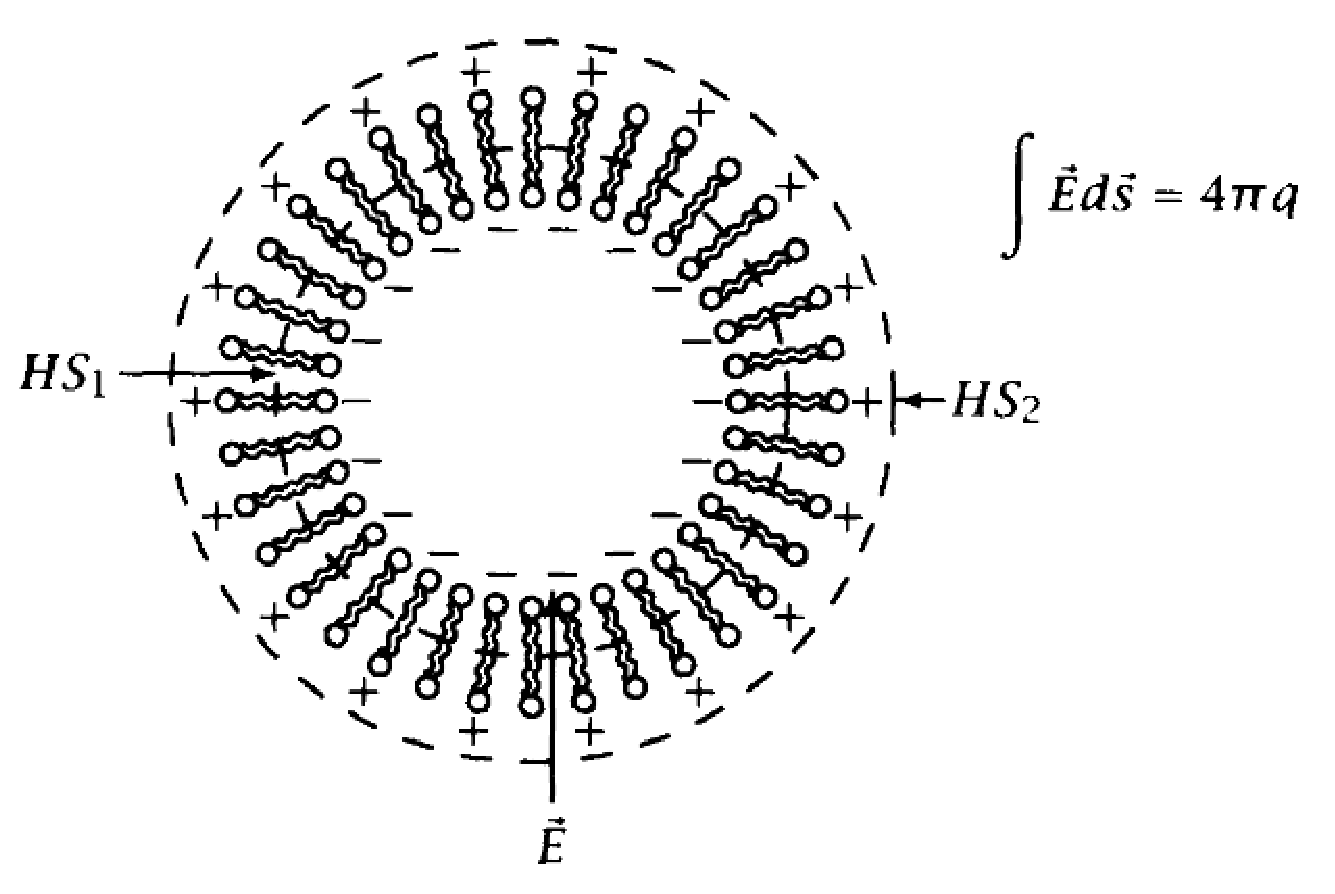
\includegraphics[height=5cm,
    angle=0]{./images/sphere_cell_02.eps}}
  \caption{spherical cells}
  \label{fig:sphere_cell_charge}
\end{figure}

For a given volume, the amount of positive charges is approximately equal to the
amount of negative charges. 
\begin{equation}
  \label{eq:1371}
  \sum z_i^A (+e) [\text{C}_i] =   \sum z_i^C (+e) [\text{C}_i] 
\end{equation}
with $z_i^A, z_i^C$ are valences of anion species, and cation species,
respectively.  This holds for any volume of biological systems, except
in the plasma membrane where the electric field is non-zero. We'll
discuss the movement of ions across the membrane via ion channels in
Sect.~\ref{sec:movement-ion-across-ion-channels}.

Another way to express the space-charge neutrality is using Gauss's
law which states that, the flux of electric field $\mathbf{E}$ through
any closed surface, of a given volume (no matter what the shape is),
is equal to $4\pi$ times the total charges enclosed in that closed
surface.
\begin{eqnarray}
  \label{eq:413}
  \int_{surface} \mathbf{E}\cdot d\mathbf{a} = 4\int_{volume} \rho dv = 4\pi Q
\end{eqnarray}
with $\mathbf{a}$ is the oriented area, $\rho$ is the charge density
(coulombs per volume) (NOTE: $\cdot$ is scalar product). This means
that
\textcolor{red}{the electric field only depends on the total charge
  the volume contains, not the shape of the volume}.

As shown in Fig.~\ref{fig:sphere_cell_charge}, the electric field
inside HS1 is non-zero, as the total charge is negative. However, the
electric field inside HS2 is zero, as the total charge now is zero.


\section{Resistance vs. Conductance}
\label{sec:resistance-conductance}

Ohm's law often uses resistance $R$ (Ohm $\Omega$) to characterize current
flows. In electrophysiology, the current flow through an ion channel is often
represented by the reciprocal of resistance, or conductance $g$ (unit:
Siemens, S).

\begin{mdframed}
EXPLAIN:
Along the cell membrane, ionic channel form parallel circuit of resistance $r_i$
with $i$ is channel index. When multiple channel opens, the new resistance
formed by these channels is $1/r_\text{total} = 1/r_i + 1/r_2 + \ldots + 1/r_n$. 

If we use conductance, the formula is simpler 
$g_\text{total}=g_1 + g_2 + \ldots + g_n$.

\end{mdframed}


The resistance of a given object depends primarily on two factors: What material
it is made of, and its shape.
\begin{equation}
R = \frac{l\rho}{A}
\end{equation}
with $l = $ length of the conductor [m], $A$ = cross-sectional area [m$^2$],
$\rho = $ electrical resistivity (specific electrical resistance) of the
material [Ohm.m].
\begin{equation}
G = \frac{A}{l}\sigma
\end{equation}
with $\sigma = 1/\rho$ = electrical conductivity [S/m].

The formula above is not exact, as it assumes the current density is totally
uniform in the conductor, which is not always true in practical situations.
However, this formula still provides a good approximation for long thin
conductors such as wires.

Another situation for which this formula is not exact is with alternating
current (AC), because the skin effect inhibits current flow near the center of
the conductor. For this reason, the geometrical cross-section is different from
the effective cross-section in which current actually flows, so resistance is
higher than expected.

\url{https://en.wikipedia.org/wiki/Electrical_resistance_and_conductance}


\section{Effective volumes}
\label{sec:effective-volumes}

In cell, a large fraction of the calcium is bound to buffers. If the binding is
assumed to be fast or instantaneous, the change in calcium concentration can be
calculated by multiplying the change (d[$\Ca$]/dt) with the so-called buffering 
fraction is $\beta$, the real amount of calcium should be $c/\beta$, defined
over the volume $V$. However, we don't use $c/\beta$ as the concentration, but
$c$ as the concentration. Then, this concentration should be defined over a 
different volume, known as {\bf effective volume} $\hat{V}$. 
\begin{equation}
  \label{eq:1412}
  c/\beta.V = c\hat{V}
\end{equation}
or
\begin{equation}
  \label{eq:1411}
  \hat{V} = \frac{V}{\beta}
\end{equation}
% part of the volume of the compartment is occupied by the buffer. So,
% it's common usually to use the effective volume, which is the real
% volume divided by the buffering factor in calculation
% \begin{equation}
%   \label{eq:1008}
%   \hat{V} = \frac{V}{\beta}
% \end{equation}
% with $\beta$ tells the fraction of volume of the species being used
% for buffering. 
E.g.
\begin{equation}
  \label{eq:1009}
  \begin{split}
    \hat{V_\nsr} &= \frac{V_\nsr}{\beta_\nsr} \\
    \hat{V_\ds} &= \frac{V_\ds}{\beta_\ds}\\ 
    \hat{V_\myo} &= \frac{V_\myo}{\beta_\myo} 
  \end{split}
\end{equation}

In non-spatial model, or in spatial model with the assumption of
stationary buffers, we can assume a constant fraction of $\ca$ buffer
capacity for the myoplasm $\beta_\myo$~\citep{williams2007pda}.

\section{Units in electrophysiology}


When performing any of the calculation between those quantities, it's
important to know their units.  Standard units are: milivolts,
miliseconds, nanofarads, nanoamperes, microsiemens (mS)
\begin{verbatim}
nF .mV/mS = nA = uS . mV
\end{verbatim}


However, in physiology, a better convention for some units is to
define them {\it per unit of surface area}. This will avoid the
geometrical difference between cells. The surface area of a neuron
might be $3\times 10^4 \mu$m$^2$, or $3\times 10^{-2}$cm$^2$.  So, the
new units are nanofarads per centimeters, nanoamperes per square
centimeters, milisiemens per square centimeters.
\begin{verbatim}
(uF/cm^2) . mV/mS = uA/cm^2 = (mS/cm^2) . mV
\end{verbatim}
The quantities that are unaffected are milivolts, miliseconds. 

So, we use $\Csc$ (nF/cm$^2$) and $R_m$ ($\Omega$.cm$^2$).

\section{How fast a reaction}
\label{sec:how-fast-reaction}

Cells are dynamic processes in which a change in cells can be of
physical or chemical origins (Chap.\ref{chap:chem-react-transp}).  
To see how fast of a chemical reaction, we use a quantity that tells
the time, counting from the starting of the reaction, at which a
certain fraction of the product has been catalyzed. The choice of the
``fraction'' will be discusses shortly. 

\subsection{Exponential time constant $\tau$ (first-order reaction)}
\label{sec:expon-time-const}

\textcolor{red}{In practice, many chemical reaction follows
  first-order kinetics}, or we can break up into a number of first-order
  chemical reactions.
As shown in eq.~\eqref{eq:415}, the current concentration of A is an
exponential function of the initial concentration $[\A]_0$. 

To see how fast/slow of such first-order reaction, they estimate the time when
the ``fraction'' of reactant to be used is 1/2; and the time point is known as
half-time constant or reaction half-time (or {\bf doubling-time constant} if we
refer to the product), i.e.
when half of the reactant has been consumed, or the product increased double.
This is denoted as $T_2$ (for product) and $T_{1/2}$ (for reactant)
\begin{equation}
  \label{eq:663}
  \begin{split}
    T_{1/2} &= \frac{\ln 2}{|k|}\; ; \; k<0 \\
    T_2 &= \frac{\ln 2}{k}\; ; \; k>0 
  \end{split}
\end{equation}
However, back to the time this concept was formulated, people don't
have calculators to find the logarithm. So, people prefer using the
{\bf exponential time constant} $\tau$, i.e. we use $\exp(t/\tau)$
rather than $\exp(kt)$. The unit of $\tau$ is unit of time.
\begin{equation}
  \label{eq:664}
  \tau = \frac{1}{k}
\end{equation}
$\tau$ is the amount of time we must wait for an e-fold increase
($e\approx 2.71$) or decrease (about 1/3 of the initial value).

\begin{framed}
  {\bf TIP}: We can think of reaction half-time as a one cell cycle (one
  generation), while exponential time constant is the triple in time.
\end{framed}

\begin{framed}
  In cell physiology, there is a different concept, though the term looks
  similar, called {\bf membrane time constant}
  (Sect.\ref{sec:membr-time-const-1}) 
\end{framed}

\subsection{Characteristic time (time scale) $\mathcal{T}$}
\label{sec:char-time-time}

For reactions whose rate of changes that are not exponential, it's hard
to find the exponential time constant. Instead, we often speak of a
``time scale'' or ``characteristic time''. It tells how fast/slow of
change of a system. At first
\begin{enumerate}
\item Find the max and min signal: $M_{max},M_{min}$
\item Find the maximum value of the slope (first-order derivative)
  of points within the range from min to max
\item Find the intersections of that slope with two horizontal line
  across the max and min signal.
\item The time between the two intersections is called the {\bf
    characteristic time} $\mathcal{T}$. 
  \begin{equation}
    \label{eq:665}
    \mathcal{T} = \frac{M_{max}-M_{min}}{\max\{\text{slope}\}} 
  \end{equation}
\end{enumerate}

{\bf Example}: The sinusoidal signal $y=\sin(\frac{2\pi t}{T})$. The
max and min value is $M_{max}=1,M_{min}=-1$. The slope is 
\begin{equation*}
  \text{slope}=y'=\frac{2\pi}{T}\cos(\frac{2\pi t}{T})
\end{equation*}
with $T$ is the period, then the maximum value of slope is
$\frac{2\pi}{T}$. Then the characteristic time is
\begin{equation}
  \label{eq:666}
  \mathcal{T} = \frac{1-(-1)}{2\pi/T} = T/\pi
\end{equation}

\subsection{Time constant and observed rate constant}
\label{sec:time-const-observ}

Suppose that a reaction is at equilibrium. Then, if the reaction is
perturbed (e.g. by a sudden change in ligand concentration); the new
equilibrium state will be reached. If the system is modeled with no
intermediate state; i.e. 2 states totally, a simple exponential time
course is enough to approximated. 
\begin{equation}
  \label{eq:843}
  \ce{A <=>[k_{12}][k_{21}] B}
\end{equation}
The rate of this process, thus, can be expressed via an {\bf observed
  time constant} $\tau$, or its reciprocal, the {\bf observed rate
  constant} $\lambda = 1/\tau$.
\begin{equation}
  \label{eq:842}
  \begin{split}
    \tau &= \frac{1}{k_{12}+k_{21}} \\
    \lambda &= k_{12} + k_{21}
  \end{split}
\end{equation}
and the exponential function is $e^{-\lambda t}$ or $e^{-t/\tau}$. 

Equilibrium will be fast ($\tau$ is small) if either the forward
($k_{12}$ is large) or the backward ($k_{21}$ is large) is fast. 



\section{Cytoplasmic resistivity}

Dendrites tend to be long and thin.
The cytoplasm has relatively low electrical resitivity
(Sect.\ref{sec:cytoplasmic-resistivity}); while the membrane has relatively high
resistivity. NOTE: Materials with low electrical resitivity enable current
through easier.



\section{Sign and Direction: Voltage and Current}
\label{sec:voltage-current}

Strictly, voltage is ``energy per unit charge'' (i.e. joules per coulomb, or
equivalent unit: volt).
Voltage is supplied by a battery, and is used by a component (light bulbs,
resistance...), but not in wires. That's why we say voltage across a component. 
Thus, the proper name for {\bf voltage} is {\bf potential difference}, i.e.
$V_m = V_a - V_b$.

Electronic currents, on the other hands, is the {\bf rate of flow of charge}.


\begin{figure}[hbt]
  \centerline{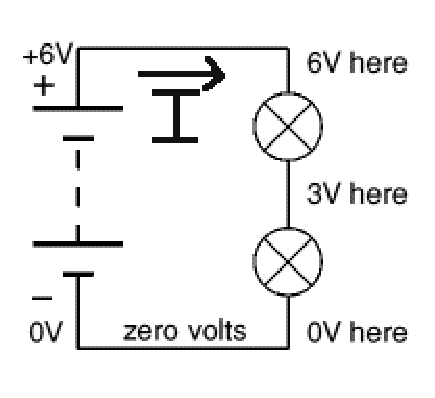
\includegraphics[height=4cm,
    angle=0]{./images/V_I_direction.eps}}
\caption{I-V in electronics}
\label{fig:V-I_elec}
\end{figure}

\subsection{Conventions in electronics}

There are two types of current: direct current (DC) and alternating current
(AC). Direct current has a constant direction, and/or possessing a voltage with
constant
polarity\footnote{\url{http://www.allaboutcircuits.com/vol_2/chpt_1/1.html}}.

In electronics, the common convention for the direction of DC current is the
direction from high voltage to low voltage (high energy to low energy). Besides,
in the common sense, the voltage is defined as the difference between the pole
with high voltage to that of low voltage so that the voltage difference is
always non-negative.

\begin{mdframed}
In electronics we rarely use the name 'potential difference'. Instead, one end
is often implicitly given the value 0(V). The point with zero volt is
often set to the negative terminal of a battery.
\end{mdframed}

In a standard copper wire, electrons are the charge carriers and drift along the
gradient of electrical potential. Even though the electrons (-) are the mobile
charge-carriers, it has long been the convention that the direction of {\it
electric current} is the flow of positive charge. As electrons always move from
the point of negative potential to points of positive potential, the current
flow is considered as the flow of ``imagined'' positive charges.  This flow of
positive charges is known as {\it conventional flow}. The direction of the flow
of electrons is thus of the opposite side of the direction of currents, or the
current go out from (+) pole, and enter (-) pole, Fig.\ref{fig:V-I_elec}.

\subsection{Conventions in cell electrophysiology}
\label{sec:conv-cell-phys}

In electrophysiology, only DC current is used. The convention described in the
previous section, however, is not that being used for studying the  electrophysiology of
the membrane\footnote{\url{http://www.tpub.com/content/doe/h1011v1/index.htm}}.
\textcolor{red}{Thus, there are four important points to know when
  studying cell electrophysiology.}

The charge carriers in electrophysiology are mainly one of the two ionic
species, $\Na$ and $\K$, and to a lesser extent $\Ca$ and $\Cl$.

\begin{itemize}
\item the intracellular terminal is cathode (-), while the
  extracellular is anode (+).

\item membrane potential is the difference between that in the
  cytoplasm w.r.t that in the extracellular, $V_m=V_i-V_o$, as shown
  in Fig. \ref{fig:Ohm_circuit}. Thus it can be positive or negative. 

So, to measure the voltage, we need two reference points. We will learn that
there has been a change in the sign convention as in the early days (pre-1980s),
$V_m=V_o-V_i$.

\item ionic membrane currents $I_X$ (with $X$ represents an ion species) are
defined with positive sign for outward direction and negative for inward ionic
current.
  
\item applied (injected) current $I_\app$ (or $I_\text{inj}$) is inward
direction yet the sign is (+), eq.
\ref{eq:1469}.
\end{itemize}

\begin{figure}[htb]
  \centerline{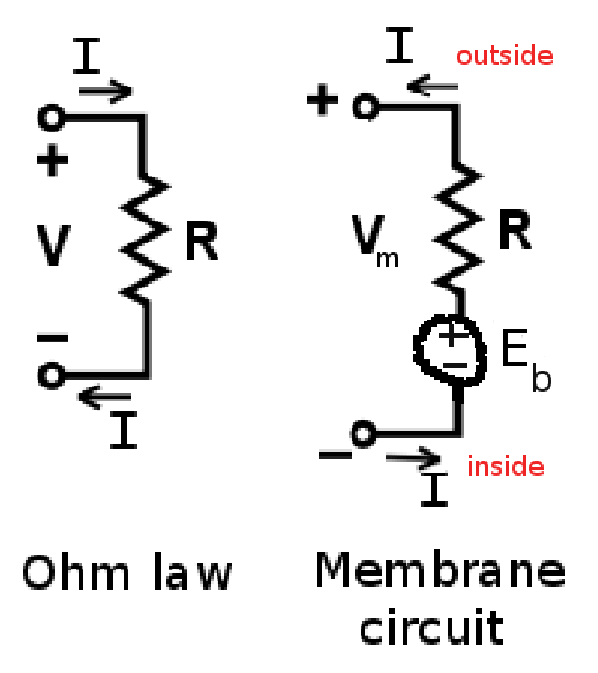
\includegraphics[height=5cm]{./images/Ohm_membrane_circuit.eps}}
  \caption{(A) Normal circuit, (B) Membrane circuit}\label{fig:Ohm_circuit}
\end{figure}



\section{The formation of reactions - Theory of absolute reaction rate}
\label{sec:form-react-theory}

% \subsection{Basic biochemistry}
% \label{sec:basic-biochemistry}

% Consider a reaction:
% \begin{center}
%   \ce{mA + nB ->[k] pC}
% \end{center}
% The reaction {\it rate
%   constant}\footnote{\url{http://en.wikipedia.org/wiki/Rate_constant}}, 
% $K$ or $\lambda$, quantities the
% speed of the reaction.  The rate equation is
% \begin{equation}
%   \label{eq:68}
%   \frac{dC}{dt} = K [A]^m[B]^n
% \end{equation}
% with [X] is the concentration of the substance X; its unit is
% [moles/volume] (or [moles/area] if the reaction occur at the
% boundary).  The {\it order of the reaction} above is $(m+n)$.  $K$ is
% the coefficient depending on the temperature and its unit depend on
% the {\it order of the reaction},


% \subsection{The formation of reactions}
% \label{sec:formation-reactions}


\begin{figure}[htb]
  \centering
  % \input{./images/state_transition_t}
  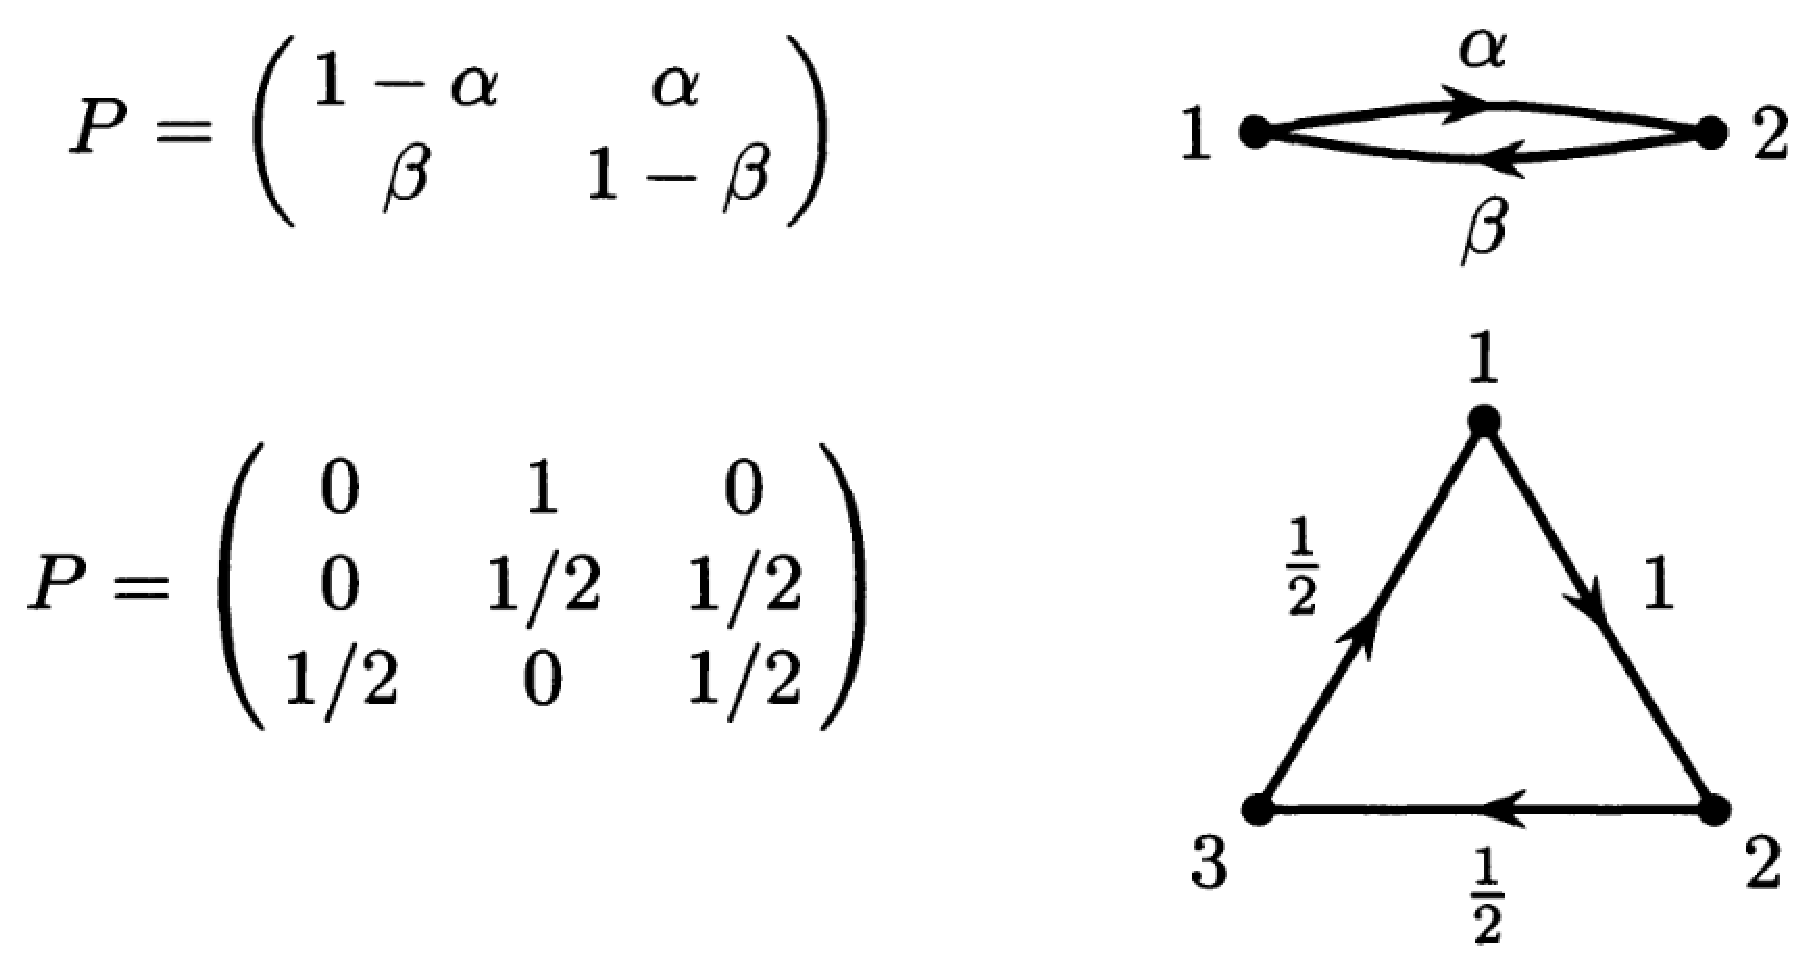
\includegraphics[height=7cm]{./images/state_transition.eps}
  \caption{State transition}
  \label{fig:state_trans}
\end{figure}

In general, chemical reactions require splitting existing chemical
bonds. To analyze such processes, it is necessary to know the
interaction energy of an atom as a function of distances to each of
its neighbors.

{\bf Example:} For simplicity, we consider the interaction
(e.g. bonding) between two molecules. As shown in Fig.
\ref{fig:state_trans}, the two molecules can be in contact
(associative state AS), or can be aparted (disassociated state
DS). Both are quite stable states. In order to jump from one state to
another, there should be an intermediate state that is very
unfavorable and unstable that we call it the {\it transition state} TS.

The energy at TS is relatively higher than those of the two stable
states (DS and AS), and we call it {\it activation energy} (or
mid-night energy). When the system's energy reach to the level of TS,
the TS is now {\it activated}.  The height from the energy at TS to
that of a stable state is, conceptually, termed the
{\it potential barrier} (or the energy barrier) and denoted as $E_A$
or $E_a$ or here we use $\Delta G_0^\#$.

\begin{comment}
  Consider two atoms (molecules) in the surface of free energy. Then,
  the path from A $\rightarrow$ B will essentially has a
  valley-shaped. It means that the reaction follows the path that has
  minimum activation energy.
\end{comment}

In reality, the bonding can be a hydrophobic tether in which two
chemical groups be in contact (or tether)(CS or AS) or disassociated
state (DS).  We consider the reversible reaction

\begin{equation}
  \label{eq:ASDS}
  AS  \xrightleftharpoons[b]{f} DS  
\end{equation}
The {\it rate constant} is relatively high in the initial ($K_0$) and
then decreases. This relation is formulated as follows ({\bf Arrhenius equation})

\begin{equation}\label{eq:Arrhenius}
  K = K_0.e^\frac{-\Delta G_0^\#}{RT}
\end{equation}
with $K_0$ (unit depending on the order of the reaction) is an
empirical factor ({\it Arrhenius-coefficient}) - the initial rate
constant, [$\Delta G_0^\#$] = Joules/mole (note: we substitute $R$ by
$k_B$ when [$\Delta G_0^\#$] = Joules/molecule).

A simple interpretation is that $K_0$ is the number of collisions per
second, and $e^\frac{-\Delta G_0^\#}{RT}$ is the probability that any
given collision will result in a reaction. Then $K$ is the number of
collisions that leads to reactions per second. This relation is
discovered by Arrhenius and hence the eq.~\eqref{eq:Arrhenius} is
called {\bf Arrhenius equation} which is closely related to van't
Hoff's equation. It's simple but describes an accurate relation that
tells the temperature dependence of the reaction
rate\footnote{\url{http://en.wikipedia.org/wiki/Arrhenius_equation}}.


{\bf REMARKS:}
\begin{enumerate}
\item $K$ is called a rate constant, yet not exactly a constant. For a
  given reaction,  it's a constant at a given temperature. However, it
  varies exponentially upon the temperature $K=K(T)$.
% \item The formula $K = K_0 e^{-\frac{\Delta E}{k_B T}}$ with $\Delta
%   E$ is the activation energy that we have studied (when dealing with
%   the number of particles passing the energy barrier) is a special
%   case of Arrhenius equation ( the unit of $\Delta E$ is Joules per
%   molecule).

\item Using {\it theory of absolute reaction rate} (aka {\it transition
    state
    theory})\footnote{\url{http://www.faqs.org/theories/A-Ac/Absolute-Reaction-Rate-Theory-of.html}},
  it is assumed that there is an equilibrium between the AS and TS
  state as given in eq.~\eqref{eq:67}. 
\begin{equation}
  \label{eq:67}
  AS
  \xrightleftharpoons[b]{f} TS \rightarrow DS  
\end{equation}
(note: since there is very few number of molecules from DS go back to
TS so we can consider it as a unidirection reaction).

The equilibrium constant for the first phase is $K^*_{eq}$ (the symbol
* refer to the activated transition state).  Its relation with the
rate constant ($K$) is derived by Wilson-Sommerfeld from kinetic
quantum theory \citep{glaser2001biophysics}.
  \begin{equation}
    \label{eq:WilsonSommerfeld}
    K = q \frac{k_BT}{h}K^*_{eq}
  \end{equation}
  with $q$ is the fraction between activated molecules which leaves to
  the right vs. to the left of the activation energy (for symmetry of
  the relations, we have $q=1$); $h = 6.62\times 10^{-34}$ (J.s) is the
  Planck's constant.

  Based on eq.~\eqref{eq:vantHoff_2}, we have
  \begin{equation}
    K = q \frac{k_BT}{h}e^{-\frac{\Delta G^*}{RT}}
  \end{equation}
and combining with eq. ~\eqref{eq:69}, the result is
  \begin{equation}
    K = q \frac{k_BT}{h}e^{-\frac{\Delta H^*}{RT}}e^{\frac{\Delta S^*}{R}}
  \end{equation}
  The temperature independent exponential part is of particular
  interest. The macromlecules, during the reaction, can get a larger (
  $\Delta S^* < 0$) or a lower ($\Delta S^* < 0$) degree of order. We
  call $ S^*$ is {\bf entropy of activation} which tells the
  conformation of the macromolecules.

  Under the conditions that the total number of molecules remains
  constant (e.g. the sum of stoichiometric numbers between the
  reactants and the products are the same), $\Delta G = 0, q=1$ and small molecules,
  the value of $K$ is

  \begin{equation}
    K = \frac{k_BT}{h} = 10^{13} s^{-1}
  \end{equation}
  at T = 300K (human body temperature).


\item The Arrhenius equation in eq. \eqref{eq:Arrhenius} is important since it not only
  describes the temperature dependence of chemical reactions, but also
  can be used to describe other time dependence quantities such as
  diffusion, kinetics of phase transition, complicated biological
  processes - at certain temperature intervals - (e.g. growth rate,
  heart rate), structural transition in biomolecule (only if there is
  a dominant free energy barrier)...

\item For a problem in which we want to know whether a time dependence
  parameter $K$ follows the Arrhenius equation or not, we often use
  {\bf Arrhenius plot}. Based on the fact that if such quantity $K$
  follows the Arrhenius equation, then 
  \begin{equation}
    \ln \frac{K}{K_0} = -\frac{\Delta G^\#}{RT} =  \frac{\Delta S^\#}{R} - \frac{\Delta H^\#}{RT} = f(1/T)
  \end{equation}
  In other words, we expect to see a straight line between (1/T)
  vs. ln(K/K$_0$) if $K$ follows the Arrhenius equation.

%   NOTE: $\Delta G^\# = \Delta H^\# - T\Delta S^\#$.

\item Using Arrhenius equation, we can calculate the life span of a
  bond possessing a specific bonding energy resisting the attack of the
  energy of thermic noise ($RT$). In that sense, we have $K =
  \frac{1}{\tau}$, and the quantity
  \begin{equation}
    \tau = \tau_0 e^{\frac{E_D}{RT}}
  \end{equation}
  will tell us how much time to cross this energy barrier (i.e. the
  bonding is broken). $E_D$ is the activation energy of a decay
  reaction. For small molecules, the values of $\tau_0$ ranges from
  $10^{-14} \rightarrow 10^{-13}$ second. And depending on the
  activation energy $E_D$, the lifespan can vary from a very short time
  ($10^{-12}$s) to very long time span ($10^5$s). 

  The {\it mean life span} is a typical variable of statistical
  thermodynamics. In DNA, the spontaneously molecular transformation,
  known as mutations, results in new residues whose stability has not
  yet been approved by natural selection. The lifespan of these
  residues can be changed by a slightly displacement of its bond
  energy. Hence, remutations (mutation on mutated residues) occur more
  often than could be expected statistically.

  Protein folding occurs in sub milli-second scale. In other words,
  normally, in protein folding, the value of $E_D$ is about
  $(1\rightarrow10)\times RT$; and in protein aggregation, the value
  of $E_D$ is $(20)\times RT$. In deed, a small change in activation
  energy, e.g. in the presence of enzyme, will lead to dramatic
  changes of the life span.


\item Even though a real biological process usually consist of a large
  number of single reactions, each with different activation energies,
  the overal process is determined by a
  {\bf simple limiting reaction}, i.e. the slowest reaction in a
  series of chemical reaction. Example:

\ce{NO2 + NO2 -> NO + NO3} (slow step)

\ce{NO3 + CO -> NO2 + CO2} (fast step)

Clearly, no matter how fast the second step can be, the overal rate
should be at the same rate of the slower step 1 since one of the
reactants in step 2 is the product of the step 1. Such kind of process
is called {\it rate limiting process}. In that sense, the straight
line of the Arrhenius plot for the slowest step will reflect the
activation energy of this rate limiting process\textit{rate limiting
  reaction}\footnote{\url{http://en.wikipedia.org/wiki/Rate-determining_step}}.
\end{enumerate}

{\bf Example}: $H_2O \xrightleftharpoons[]{K_d} H^+ + OH^-$

$K_d = 2.5\times 10^{-5} s^{-1}$

$\tau_d = 11 hours$

$pK = pH - \log \frac{[OH^-]}{[H_2O]}$


\section{Fickian motion: no viscosity}
\label{sec:transport-process}

This section deals with the movements of molecules which is the basic
behavior of life entities. Even though there is still no universally
accepted theory of the liquid state, one can account for the overall
behavior of liquids through the formal treatment of diffusion and
viscosity (the quantity that describes the fluid's resistance to
flow). Here, we just mention the basic movement, diffusion, and one
measure - viscosity. For a complete description, read
Sect.\ref{chap:appendix-b}. 


The direction of the force of atomic bombardment is constantly changing, and at
different times the particle is hit more on one side than another, leading to
the seemingly random nature of the motion. This was called {\bf Brownian motion}
(Sect.\ref{sec:Brownian-motion}).
\url{http://en.wikipedia.org/wiki/Brownian_motion}


\subsection{Diffusion: Particles in water}
\label{sec:diffusion-particles}


From observing the Brownian motion (Sect.\ref{sec:Brownian-motion}), Einstein
pointed out that the water molecules (because of their smaller sizes) are more
mobile than the pollen particles. Hence, it is valid to think in terms of the
water molecules that hit the pollen particles, but not the reverse.

\begin{figure}[hbt]
  \centerline{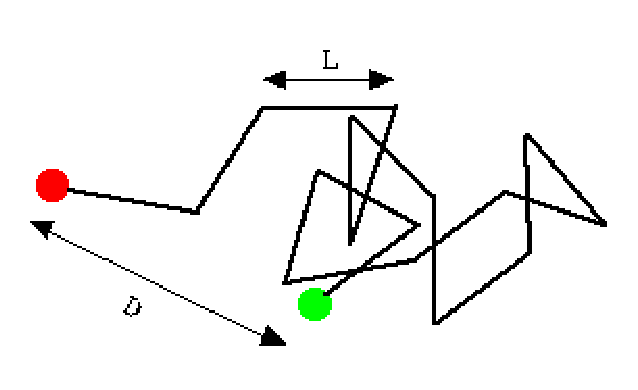
\includegraphics[height=5cm,
    angle=0]{./images/random_walk.eps}}
\caption{Random walk}
\label{fig:random_walk}
\end{figure}

Einstein's formula has two parts:
\begin{enumerate}
  \item relates the diffusion coefficient to the mean
square displacement of a Brownian particle: to determine how far a Brownian
particle travels in a given time interval.

NOTE: Classical mechanics is unable to determine this distance because of the
enormous number of bombardments a Brownian particle will undergo, roughly of the
order of $10^{21}$ collisions per second.
  
  \item relates the diffusion coefficient to measurable physical quantities.
  
In this way Einstein was able to determine the size of atoms, and how many atoms
there are in a mole (i.e. Avogadro's number), or the molecular weight in grams,
of a gas
\end{enumerate}
\textcolor{red}{We will focus on the first part.}
It requires certain number of assumptions:
\begin{itemize}
  \item conservation of particle number
  \item the increment of particle position in an unrestricted one-dimensional
  space (x), denoted as $\Delta$, is a random variable.
  
The probability density function $\phi(\Delta)$ is used to describe the relative
likelihood for this random variable $\Delta$ to take on a given value.

\end{itemize}


When we examine the movement of a specific particle, we can divide its
trajectory into small straight paths. In that sense, the particle
moves from point to point in an essentially ballistic manner. Further,
if each jump is independent from the history jumps, the movement
process is said to be stochastic and the movement themselves is said
to describe a {\bf random walk}, as shown in
Fig.~\ref{fig:random_walk}.  

Assuming after $n$ small displacement of length $L$, and the particle
move in a straight line, the total displacement would be $r=nL$
However, due to the randomness in the direction of the movement
(sometimes forward, sometimes backward, sometimes to the left,
sometimes to the right...), the particle have displaced a distance
\begin{eqnarray}
  \label{eq:237}
  r = \sqrt{nL}
\end{eqnarray}
In general, if the particle moves randomly, with each displacement of
length $r_i$, then the square of the average displacement $\vec{r}^2$,
is a good measure of the Brownian motion.
\begin{equation}
  \label{eq:70}
  <\overrightarrow r^2> = \frac{\sum_{i=1}^n r_i^2}{n}
\end{equation}
with the trajectory is projected on an arbitrary
axis\footnote{\url{http://mahalanobis.twoday.net/stories/210704/}}. The
classical results showed that, in the absence of any directional bias,
the mean of distance travelled in any number of steps, $n$, is zero,
i.e. $<\overrightarrow{r}> = 0$.


The density (i.e. the number of particles per unit volume) $\rho$
changes in a Taylor series
\begin{equation}
\rho(x, t+\tau) = \rho(x, t) + \tau \frac{\partial \rho(x)}{\partial t}
\end{equation}
\ldots
\begin{equation}
\frac{\partial \rho}{\partial t} = \frac{\partial^2 \rho}{\partial x^2} \times
\int^{+\infty}_{-\infty} \frac{\Delta^2}{2\tau} .\phi(\Delta)d\Delta + \text{
higher-order even moments}
\end{equation}
with the diffusion coefficient $D$ is
\begin{equation}
D = \int^{+\infty}_{-\infty} \frac{\Delta^2}{2\tau} .\phi(\Delta)d\Delta 
\end{equation}

The density of the Brownian particle satisfies the {\bf diffusion equation}
\begin{equation}
\frac{\partial \rho}{\partial t} = D \frac{\partial^2 \rho}{\partial x^2}
\label{eq:Einstein_diffusion_eq} 
\end{equation}
Assuming the system with $N$ particles starts from the origin at $t=0$, the
solution of the above equation is
\begin{equation}
\rho(x, t) = \frac{N}{\sqrt{4\pi D t}} e^{-\frac{x^2}{4Dt}}
\end{equation}

This allows Einstein to calcualte the moments
\begin{itemize}
  \item The first moment (mean) = 0 (as the Brownian particle is equally likely
  to move to the left as it is to move to the right)
  
  \item The second-moment (variance) is $\bar{x^2} = 2Dt$ (which is the mean
  squared displacement in terms of time elapsed $t$ and the diffusion constant $D$)
\end{itemize}

Consider in a given environment, the diffusion coefficient (or simply
diffusivity) of the particle is $D$ [cm$^2$.s$^{-1}$] in 3-dimension,
for a stochastic process, the mean squared displacement, within a
period of time t, of a particle is
\begin{equation}
  \label{eq:Einstein.1905}
  <\overrightarrow r^2> = 6Dt
\end{equation}(discovered by Einstein in 1905)

Different environment causes dramaticaly difference in travelled
distance of the particle. For example, the distance diffuse (during
the same time) in liquid is 10cm, while in solide is $10^{-1}$cm.

\begin{table}[hbt]
  \begin{center}
  \begin{tabular}{cc}
\hline
    D[cm$^2$.s$^{-1}$] & environment \\
\hline
$D=10^{-9}$ &  in solid \\
 $D=10^{05}$ & in water \\
$D=10^{-1}$ & in gas \\
\hline
  \end{tabular}
  \end{center}
  \caption{Diffusion coefficient}
  \label{tab:Diffusion}
\end{table}


Now, we consider a real-wold example of transmission in biological
environment.

{\bf Example}: Small membrane-bound vesicles deliver neurotransmitter
to the pre-synaptic membrane of nerve axons.  If the vesicle travels
in a 3D-manner, it takes a long time to reach the pre-synaptic
membrane that travelling in one dimension. We examine two cases.

\subsection{1D diffusion: Fick's first law}
\label{sec:1d-diffusion}

\begin{figure}[hbt]
 \centerline{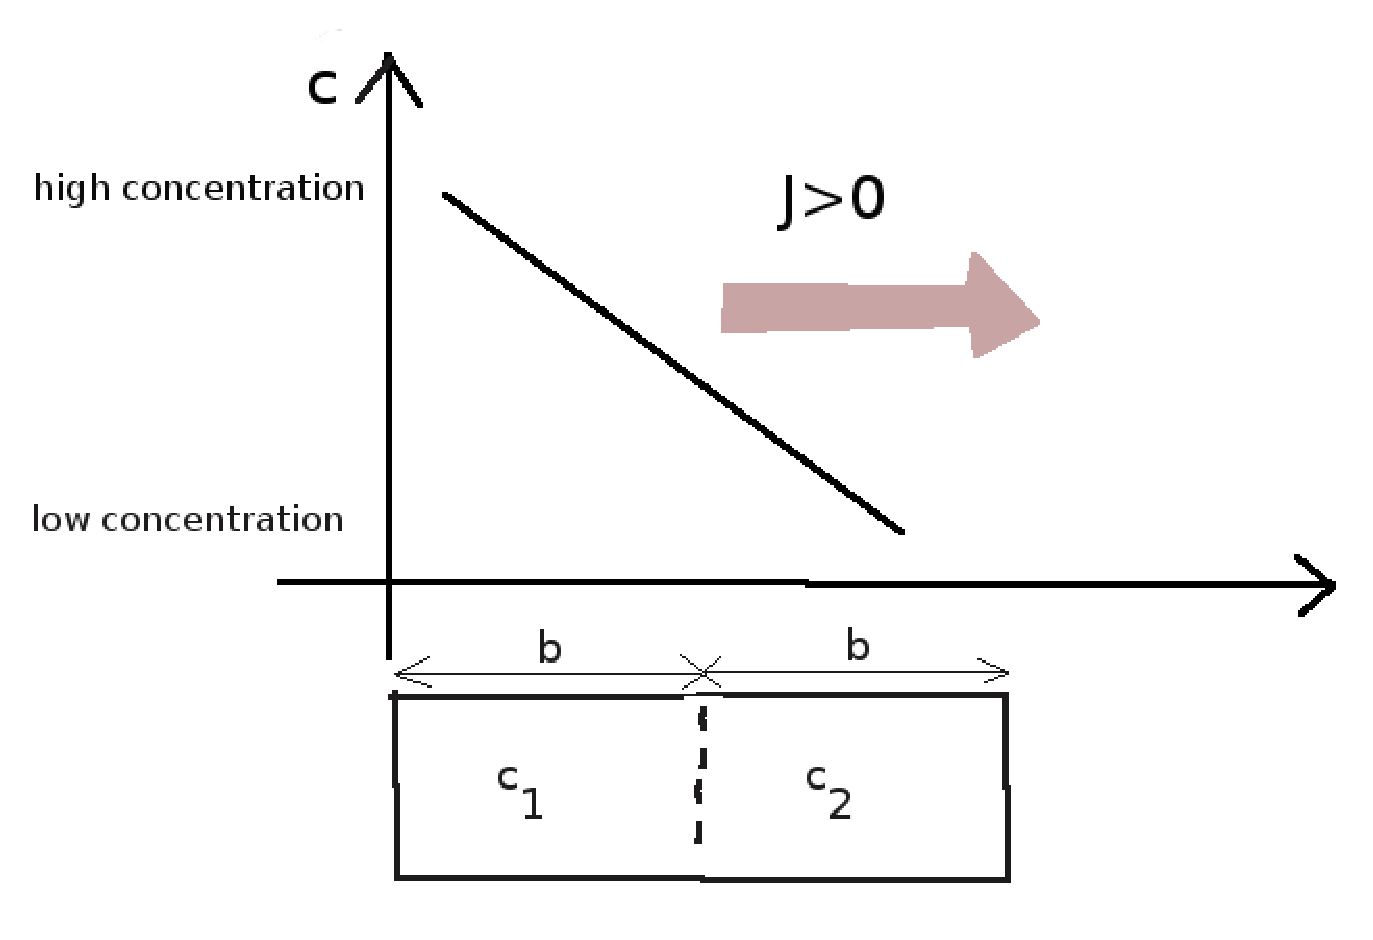
\includegraphics[height=7cm]{./images/Fick_law.eps}}
\caption{The illustration for Fick's law}
\label{fig:Fick_law}
\end{figure}

The cell creates protein microtubules that lie along the direction of
the axis of the axon to guide the passage of the vesicles. Under this
scenario, to quantitatively describe the diffusion. A conceptual
approach is to examine the situation in which the movement is along
the axis of a cylinder having a cross-section of unit area. Suppose
that the cylinder is divided into imaginary slabs of thickness $b$,
which is equal to the length of a single diffusive jump.

We consider two successive imaginary chambers of length $b$, chamber
one on the left side, as shown in Fig.~\ref{fig:Fick_law}. Let's $c_i$
denotes the concentration of molecules [per cross-section's area] in
chamber $i$, then the number of molecules in chamber $i$ is
\begin{equation}
  \label{eq:71}
n_i = c_ib  
\end{equation}
and that $c_1 > c_2$. Let's $f$ denotes the frequency with which the
particles make their jumps. There are two possible direction of jumps,
left or right, with equal probability (i.e. 1/2). Hence, the number of
particles move from the chamber 1 to chamber 2 is $\frac{1}{2}n_1f$,
and the number of particles move from the chamber 2 to chamer 1 is
$\frac{1}{2}n_2f$. 

Assuming the positive direction of the axis is from left to right,
then the flux $J$ of particles across the imaginary plane that devide
the two chambers per a unit time is
\begin{equation}\begin{split}
    J &= \frac{1}{2}n_1f - \frac{1}{2}n_2f \\
   &= \frac{1}{2}fb \left (c_1 - c_2 \right) \\
   &= -\frac{1}{2}fb \left (c_2 - c_1 \right) \\
    &= -\frac{1}{2}fb^2 \frac{\partial c}{\partial x} 
  \end{split}
\end{equation}

The examining context is for 1D diffusion, then the simple
diffusion coefficient
\begin{equation}
  D =\frac{ <\overrightarrow r^2>}{time} = <\overrightarrow
  r^2>.f = \frac{1}{2}b^2f
\end{equation}

Finally, we have the formula 
\begin{equation}
  J= -D \frac{\partial c}{\partial x}
\end{equation}
which is called {\bf Fick's First Law} (for a single dimension
movement). As we're assuming $c_2 < c_1$, and the gradient is the new
value minus the old value, the negative sign of the right side
indicates that the flux is flowing from left to right, or in other
words, in the direction of lower concentration.

In 2 or more dimension, we use
\begin{equation}
J = -D \nabla c
\end{equation}

\subsection{3D diffusion: Einstein formula}
\label{sec:3d-diffusion}

Now, for a more general case, a random jump can
move in 3D space, without the friction and collision, we have the
classical Newton equation
\begin{equation}
  m \frac{d^2\overrightarrow r}{dt^2} = \overrightarrow F
\end{equation}
In the general case, with friction force $-\xi \frac{d\overrightarrow
  r}{dt}$ and force due to collision $\overrightarrow R$, we have
\begin{equation}
  m \frac{d^2\overrightarrow r}{dt^2} =\overrightarrow F - \xi
          \frac{d\overrightarrow r}{dt} + \overrightarrow{R} 
\end{equation}
with $\xi$ is the {\it friction coefficient} (or drag coefficient)
\begin{equation}
  \xi = \frac{k_BT}{D}
\end{equation}
is the {\bf Einstein's formula}. 

\subsection{3D diffusion: Stoke's formula}

However, if the particle is a spherical shape of radius $r$, then the friction
coefficient is formulated as ({\bf Stokes' formula})
\begin{equation}
  \xi = 6\pi\eta r
\end{equation}
with $\eta$ is the viscosity [dyne.s.cm$^{-2}$] = [Poise] = [P] (Jean
Louis Poiseuille).

Finally, we learn this very important formula
({\bf Einstein-Stoke's formula}) for the diffusion coefficient in 3D
space:
\begin{equation}
  D = \frac{k_B T}{6\pi \eta r}
\end{equation}

{\bf REMARKS}:
\begin{enumerate}
\item Diffusion occurs due to the non-zero gradient of concentration

\item Flux $J$ is proportional to diffusion coefficient $D$.

\item The diffusion coefficient depends on the temperature, the
  viscosity and the size of the particle.
\end{enumerate}


\section{Navier-Stock equation: particles in viscous fluid (viscosity)}
\label{sec:viscosity}
\label{sec:navier-stock-equation}

Viscosity is a quantity that measures the resistance of a fluid to
flow. Then, to describe the motion of a fluid substance, we use
{\bf Navier-Stokes equations}. This is a set of differential equations
that describes how velocity $\mathbf{v}$, pressure $p$, temperature
$T$ and density $\rho$ are related. However, they do not explicitly
establish the relation among the variables of interest (e.g. velocity
$v$ and pressure $p$), but their rate of changes (e.g. $dv$ and
$dp$). These equations were derived independently by Navier in France
and Stokes in England\footnote{\url{http://www.grc.nasa.gov/WWW/K-12/airplane/nseqs.html}}.

For a particle of spherical shape of radius $r$ to move within a
fluid of  viscosity coefficient $\eta$ (eta), and the
temperature is $T$, then the displacement (for a single particle)
within a time interval $\Delta t$ is now

\begin{equation}
  <\overrightarrow r^2> = \frac{k_BT \Delta t}{3\pi \eta r}
\end{equation}
which is the {\bf Einstein-Smoluchowski} formula. This will alows us
to compute the time for a single particle crossing a certain distance
by diffusion.

The eq.\ref{eq:Einstein_diffusion_eq} is assumed in the osmotic pressure
experiment A similar formula can be achieved if particles are in a viscous fluid
(viscosity $\mu$ - particle's mobility in the fluid) in a gravitational field
($g$ = gravitational acceleration). There are two regions:
lower part of higher concentration, and upper part with lower concentrations. Gravity tends to make
the particles settle, whereas diffusion acts to homogenize them, driving them
into regions of smaller concentration.
\begin{enumerate}
  \item downward speed under the action of gravity: $v = \mu mg$, with $m$ =
  particle's mass
  
  \item the mobility of a particle of spherical shape  with radius $r$ follows
  the George {\bf Stoke's equation}:
\begin{equation}
\mu = \frac{1}{6\pi \eta r}
\end{equation}
with $\eta$ = dynamic viscosity of the fluid.
\end{enumerate}
 In a state of dynamic equilibrium, the particles are distributed according to
the barometric distribution
\begin{equation}
\rho = \rho_o e^{-\frac{mgh}{k_BT}}
\end{equation}
with $\rho - \rho_o$ = the difference in density of particles separated by a
height difference of $h$.
%\subsection{Background}
\subsection{Advection operator, convection operator}
\label{sec:background}

{\it advection operator}: 

The word {\it advection} refers to the horizontal transfer/movement of
a body of atmosphere or fluid. In Cartesian coordinate, the {\it
  advection operator} is 
\begin{equation}
  \label{eq:73}
  (\mathbf{v}.\nabla)(*) = u\frac{\partial}{\partial x}(*) +
  v\frac{\partial}{\partial x}(*) + w\frac{\partial}{\partial x}(*) 
\end{equation}
with $\mathbf{v} = (u,v,w)$ is  the fluid's velocity in 3D-space.  The
advection operator is not simple to solve numerically.

{\it convection operator}: Convection is the most general term to
refer to the movement of molecules in a fluid.

Now, consider a quantity $\psi = \psi(\mathbf{x},t) $ is a physical quantity
that can change in time and space. $psi$ can be temperature or
chemical concentration, etc. Then, we have
\begin{equation}
  \label{eq:74}
  \frac{d}{dt}\psi = \frac{\partial \psi}{\partial t} + \nabla \psi
  \frac{\partial \mathbf{x}}{\partial t}
\end{equation}

If the path $\mathbf{x}(t)$ is chosen to have a velocity equal to that
of the fluid, then
\begin{equation}
  \label{eq:75}
  \frac{\partial \mathbf{x}}{\partial t} = \mathbf{v}
\end{equation}
Then, we have
\begin{equation}
  \label{eq:76}
    \frac{D\psi}{Dt} = \frac{\partial \psi}{\partial t} + \mathbf{v} .\nabla \psi  
\end{equation}
with $\psi$ can be a scalar or a vector and $\nabla \psi$ then is a
gradient or a tensor derivative, respectively. We call this
{\it convective derivative}.  The first term of the right-hand side is
the ordinary Eulerian derivative (the change at a point w.r.t. time)
and the second term represents the change of a quantity w.r.t
position.

% \begin{equation}
%   \label{eq:72}
%   \frac{D}{Dt}(*) = \frac{d}{dt}(*) + (v.\nabla)(*)
% \end{equation}

\subsection{Euler equations}

{\it Euler equation}: Euler equation describes how the velocity
$\mathbf{v}$, pressure $p$ and density $\rho$ are related. This is a
set of coupled differential equations and can only be solved
numerically. Our world has 3 spatial dimension (up-down, left-right,
fore-aft) and one time dimension. Euler equations have
\begin{enumerate}
\item one time-dependent equation for conservation of mass

  As the fluid is moving, the definition of mass is a little
  tricky\footnote{\url{http://www.grc.nasa.gov/WWW/K-12/airplane/mass.html}}\footnote{\url{http://www.grc.nasa.gov/WWW/K-12/airplane/mass.html}}. Let's consider an amount of fluid pass through a surface of
  area A at velocity $\mathbf{v}$ in some amount of time $t$. Then the
  volume $V$ of the fluid is defined to be
\begin{equation}
  \label{eq:78}
  V = A\times \mathbf{v} \times t
\end{equation}
Then, a mass at point ``a'', $m_a$, is simply the density $\rho$ times
the volumes at ``a''.
\begin{equation}
  \label{eq:79}
  m_a = (\rho \times A\times \mathbf{v} \times t)_a
\end{equation}
Similarly, at another point ``b'', the mass is
\begin{equation}
  \label{eq:80}
  m_b = (\rho \times A\times \mathbf{v} \times t)_b
\end{equation}
Based on the conservative of mass, we have
\begin{equation}
  \label{eq:81}
 (\rho \times A\times \mathbf{v} \times t)_a = (\rho \times A\times \mathbf{v} \times t)_b
\end{equation}
Since the time period is independent of location, we have
\begin{equation}
  \label{eq:82}
  (\rho \times A\times \mathbf{v}) = const
\end{equation}

\item three time-dependent equations for conservation of momentum
\end{enumerate}

\subsection{Navier-Stokes equation}

{\it Navier-Stokes equation}: Navier-Stokes equations is an extension
of the Euler equations when a new quantity, {\it viscosity} of the
fluid, is taken into account.

Navier-Stokes equation is based on the assumption that fluid is made
of continuum substance, not being made of discrete particles. Second,
all the field of interest like pressure ($p$), velocity ($v$), density
($\rho$), and temperature ($T$) are differentiable.  Further, the
equation is built based on the basic principles of conservation of
mass, momentum and energy.

To measure the change of a quantity, one can measure in two ways:
\begin{enumerate}
\item measure the change on a fixed point in space as the particles of
  the fluid pass by: we call it {\it Eulerian derivative}

\item measure the change of that quantity by following a parcel of
  fluid along its streamline: we call it {\it convective derivative}.
\end{enumerate}

The most general form of the Navier-Stokes equation is

\begin{equation}
  \frac{\partial \mathbf{v}}{\partial t} + (\mathbf{v}. \nabla) \mathbf{v} = \frac{\nabla p}{\rho} + \nu \Delta^2\mathbf{v} + \mathcal{F}_{body}
\end{equation}
where $\mathbf{v}$ [m.s$^{-1}$] is the flow velocity vector, $\nu$
[N.s.m$^{-2}$] is the kinematic viscosity, and $\mathcal{F}_{body}$ is the body
forces acting on the fluid.

\subsection{Special cases}
\label{sec:special-cases}


For constant flow, the first term of the left-hand side vanish.  The
second term can be neglible for favourable ratios of object size (the
term $(\mathbf{v}. \nabla)\mathbf{v}$ is of order $\mathbf{v}^2/r$,
where $r$ is the characteristic length of the object or conduit and
the term $\nu \Delta^2\mathbf{v}$ is of order $\nu
\mathbf{v}/r^2$). The ratio
\begin{equation}
  \frac{(v.\nabla)v}{\nu \Delta^2v} = order \left(  \frac{vr}{\nu}        \right)
\end{equation}
The quotient in the final parentheses is the Reynolds number
\begin{equation}
  R = \frac{rv\rho}{\eta} = \frac{vr}{\nu}
\end{equation}
where $r$ is the characteristic streaming distance, $v$ is the flow
velocity, $\eta$ is the dynamical viscosity and $\rho$ is the density
of medium.
\begin{itemize}
\item If R $\gg$ 1, it is inertial motion (depend on $m
  \frac{d^2R}{dt^2}$) which means that the motion is controlled by its
  mass (e.g. human $R=10^6$).
\item If R $\ll$ 1, it is diffusion motion (depend on $\xi, R, D$)
  which means that motion of small particles (e.g. bacteria) is
  controlled by the collision (e.g. bacteria $R=10^-5$)
\end{itemize}

REMARKS: In CHARMM, the friction coefficient is defined as $\xi = m \gamma$
with m is the mass of molecule and $\gamma$ is the damping coefficient
(frequency of collision). $[\gamma] = \frac{1}{S}$

Example:

\begin{itemize}
\item Amino acid: mass $m = 10^{-22}$g, $a$ = 5\AA, $\gamma \approx$ 50
  ps$^{-1}$, $\tau = \frac{1}{\gamma} \approx 10^{-14}$ s
\item Bacteria: mass $\eta = 0.01$ Poise, $m = 10^{-12}$g, $a = 10^-4$ cm,
  $\gamma \approx 20 \mu$ s$^{-1}$, $\tau = \frac{1}{\gamma} \approx
  10^{-7}$ s.
\end{itemize}

For more information, read Appendix \ref{chap:appendix-b}.


\section{Average molecular kinetic energy}


\url{http://hyperphysics.phy-astr.gsu.edu/hbase/kinetic/molke.html}



%%% Local Variables: 
%%% mode: latex
%%% TeX-master: "thermo-stat"
%%% End: 
%%
%% AppendixB.tex
%% Login : <hoang-trong@hoang-trong-laptop>
%% Started on  Thu Jul  9 15:16:16 2009 Hoang-Trong Minh Tuan
%% $Id$
%% 
%% Copyright (C) 2009 Hoang-Trong Minh Tuan
%%

% \chapter{Appendix B}
\chapter{Movement of particles}
\label{chap:appendix-b}

\section{Movements (Mortility) of cells}

\begin{framed}
In all cases, organisms with typical linear dimension $R$ in the range of
0.5$\mum \le R \le 10\mum$ can swim with the speeds of $v \approx 10-100\mum/s$,
thus the Reynolds number Re=$\rho.v.R/\eta$ ($\rho$ and $\eta$ are the liquid's
density and viscosity) are vanishingly small ($\le 10^{-3}$ in water).
\end{framed}

Micro-organisms use a variety of strategies to generate motion with low-Re
propulsion, i.e. by rotating or beating one or more flagella. A wild-type {\it
Escherichia coli} cell (of size $\sim 1\mum \times 2\mum$ spherocylinder) has
six to ten 6-10$\mum$ long helical flagella. For each bundle, the flagella can
rorate clockwise (CW) (viewing from flagella to cell body), they can propel the
cell forward in a straight run. Each new re-bundling, a new run is generated in
an essentially random direction, i.e. {\it random walk}.

\begin{framed}
Tracking cell movement is laborious, i.e. need over $10^2$ cells on average, and
thus limiting statistical accuracy. Also, 3D tracking requires speciallized
equipments, thus typically results are presented in 2D projections, which
further limits the statistical accuracy (as cells move out of the imaging
plane) \citep{martinez2012}. 
\end{framed}

Techniques for tracking movements involves: differential dynamic microscopy
(DDM) \citep{martinez2012}.

\section{Movements of particles}
\label{sec:movements-particles}

% In nature, transport (mass transfer) occurs in fluid through the
% combination of advection and diffusion.

{\it Environmental fluid mechanics} is the field studying natural
process that change concentrations. The change in concentrations of a
substance can be due to either (1) the movement of that substance from
one location to another, or (2) the substance is transformed into
another substance. Accordingly, these processes are classified into 2
broad groups: {\it transport} and {\it transformation}. The two
primary modes of transport in environmental fluid mechanics are
{\it advection} (transport associated with the flow of fluid (or air
in the case of gas mechanics)) and {\it diffusion} (transport
associated with random motions within the fluid).  With
transformation, there are also two primary modes: {\it physical}
(transformation caused by physical laws, e.g. radioactive decay), and
{\it chemical} (aka {\it reaction} - the transformation caused by
chemical or biological reactions, e.g. dissolution and respiration).

\subsection{Expressing concentration}
\label{sec:expr-conc}

To know that a substance change and to evaluate how much a chemical is
present in any region of a fluid, the fundamental quantity called
{\it concentration} is used. There are various ways to define the
concentration, and the measure chosen is just the matter of
taste. However, the very important point is to choose the measure of
concentration whose units are consistent with the equation (normally
PDE) used to predict fate and transport.

Mathematically, the concentration $C$ is the ratio of the mass $M_i$
of the substance $i$ to the total volume $V$ of the mixture.
\begin{equation}
  \label{eq:167}
  C = \frac{M_i}{V}
\end{equation}
with the common unit of concentration is [mg/l], [kg/m$^3$], or
[lb/gal]. 

For one- or two-dimensional problem, the concentration can also be
expressed as the mass per unit segment length (or per unit area).
\begin{equation}
  \label{eq:216}
   conc= \frac{M_i}{l}; conc = \frac{M_i}{S}
\end{equation}
In some situation, instead of using {\it concentration}, a related
quantity - the {\bf mass fraction}, $\chi$, the ratio of the mass of a
substance $M_i$ to the total mass of a mixture $M$ (including the mass
of component substances) is used
\begin{equation}
  \label{eq:167}
  \chi = \frac{M_i}{M}
\end{equation}
which is unitless, but is often expressed using mixed units,
e.g. [mg/kg], [parts per million (ppm)], [parts per billion (ppb)].

{\bf CAUTIOUS}: In dilute aqueous system, at the density of pure water
at $4^0$C as 1g/cm$^3$, making values for concentration in [mg/l] and
mass fraction in [ppm] are identical. However, in other solutions,
[ppm] and [mg/l] are not identical.

Another popular concentration measure used by chemists is the {\bf
  molar concentration} $\theta$ which is defined as the ratio of the
number of moles $N_i$ of a substance $i$ to the total volume $V$ of the
mixture
\begin{equation}
  \label{eq:167}
  \theta = \frac{N_i}{V}
\end{equation}
whose unit is [mol/l] or [$\mu$mol/l]. 

{\bf NOTE}: The atomic weight of an atom is reported in the Periodic
table in unit [g/mol], and one mole has  $6.023\times 10^{23}$
molecules. 



\subsection{Dimensional analysis}
\label{sec:dimensional-analysis}

Before developing the equations for different movements of particle,
we should learn a very powerful analytical technique called {\bf
  dimensional analysis}.

The concept behind dimensional analysis is that any process can be
represented by some parameters, usually in the form of {\it
  dimensionless variables}, to describe the process at all scales (not
just the scales we measure in the laboratory or the field). This
method is based on the {\bf Buckingham $\pi$-theorem}.

Consider a process that can be represented by $m$ variables whose
units are generated from $n$ ($m\ge n$) different physical dimensions
(length, time, mass, temperature, etc.)  Then, there are $(m-n)$
independent non-dimensional groups that can be formed from these
variables. Then, such system can be fully represented by these $(m-n)$
dimensionless variables. Mathematically, an equation involving $m$
variables can be equivalently rewritten as an equation of $(m-n)$
dimensionless variables. $n$ is called the
{\it number of fundamental dimensions} used.

The question is
\textcolor{red}{``how to find out these $(m-n)$ dimensionless
  variables from the given variables?''}
- Let's take a look at this example.

{\bf Example}: Three variables (A,B,C) with two dimension (L,T) as
given A in unit of [L/T], B in unit of [T$^2$], C in unit of
[LT]. Then we need only one dimensionless variable $\pi$ created by
\begin{equation}
  \label{eq:190}
  \pi = \frac{AB}{C}
\end{equation}
In the next section, there is a practical example for this method.

Once we have these $(m-n)$ dimensionless variables, these variables
are related to each other according to
\begin{equation}
  \label{eq:175}
  \pi_1 = f(\pi_2, ...,\pi_i,...,\pi_{m-n})
\end{equation}



\subsection{Diffusion}
\label{sec:diffusion}

The fundamental quantity in the study of diffusion is {\bf flux} -
denoted by $J$, i.e. the amount of a substance passing across a
cross-section area in a unit of time. Thus, the SI unit for flux is
mol.m$^{-2}$.s$^{-1}$.

\subsubsection{Fickian diffusion}
\label{sec:fickian-diffusion}


Diffusion refers to the transport of particles in a tilt fluid and
does not necessarily follow fluid particles. Diffusion has 2
properties: (1) random from nature, (2) transport from regions of high
concentration to another region of low concentration, with an
equilibrium state of uniform concentration.


Now, what is the {\bf diffuse flux equation}? - For didactic purposes,
we examine only one component of the 3D motion: motion left or right
along the $x$-axis. Consider a box divided into two chambers with the
mid-line is at $x=0$ as the boundary, as shown in
Fig.~\ref{fig:diffusion-chamber}, the mass of particles on the left
chamber as $M_l$, mass of particles on the right chamber as $M_r$.
The probability (transfer rate per unit of time) that a particle moves
across the boundary are the same for each chamber and is $k$, with
unit [time$^{-1}$].  Without any external factors, based on the
property of diffusion, after a period of time $\delta t$, the
distribution of particles will be uniform, i.e. half of the particles
stays on the right and half stays on the left.

\begin{figure}[hbt]
 \centerline{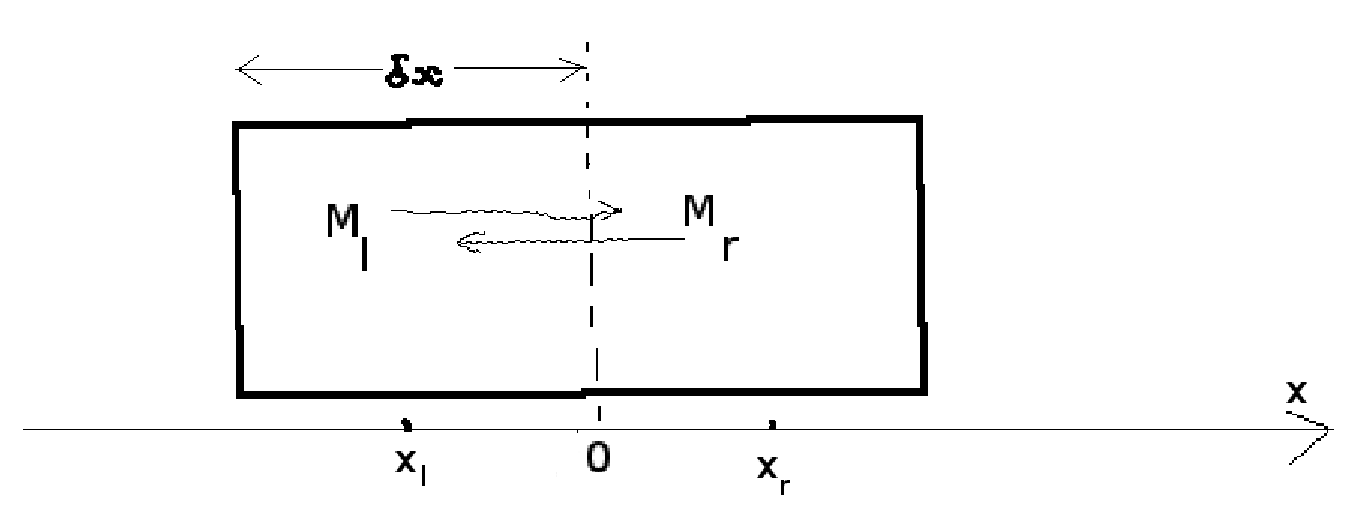
\includegraphics[height=5cm]{./images/diffusion_chamber.eps}}
 \caption{Demonstration the diffusion in closed chambers}
\label{fig:diffusion-chamber}
\end{figure}


Now, we examine the flux $J_x$ of particles passing a unit of area
(i.e. passing a single line) in a single unit of time, given the
positive direction is to the right direction. This change is caused by
the moving right of particles from the left chamber and the moving
left of particles in the right chamber.
\begin{equation}
  \label{eq:168}
  J_x = k(M_l-M_r)
\end{equation}
In order to know the total mass flux rate, we need to expand the line
to a surface $A$ and then expanding it to a volume $V$.  The flux
across a cross-section area $A$ is $J_xA$.


Assuming the volume of each chamber is $V=\delta x \delta y \delta z$,
the concentrations on each side can be written as
\begin{equation}
  \label{eq:169}
  \begin{split}
      C_l &= \frac{M_l}{\delta x \delta y \delta z} \\
      C_r &= \frac{M_r}{\delta x \delta y \delta z}
  \end{split}
\end{equation}
with $\delta x$ is the width, $\delta y$ is the breadth, $\delta z$ is
the height of the volume. 

Assuming that $\delta y \delta z = 1$, then $J_x$ represents the
\textcolor{blue}{flux in the $x$-direction per unit of cross-section
  area},
i.e.  perpendicular to $x$.  Consider the location of each chamber is
at the middle of it, then, the gradient in concentration can be
written in the form of finite difference approximation
\begin{equation}
  \label{eq:170}
  \frac{dC}{dx} = \frac{C_r-C_l}{x_r-x_l} = \frac{M_r-M_l}{\delta x (x_r-x_l)}
\end{equation}
Physically, $\delta x$ is
the average step along the $x$-axis taken by a molecule in the time
$\delta t$, or  $\delta x = (x_r-x_l)$. Then we have
\begin{equation}
  \label{eq:171}
  (M_l-M_r) = - (\delta x)^2 \frac{dC}{dx}
\end{equation}
substitute it into eq.~\eqref{eq:168}, then
\begin{equation}
  \label{eq:172}
  J_x = -k(\delta x)^2 \frac{dC}{dt}
\end{equation}

Based on the dimensional analysis,  $q$ cannot depend on an arbitrary
$\delta x$, we must assume that $k(\delta x)^2$ is a constant, which
is known as the {\bf diffusion coefficient}, denoted by $D$. Finally,
we have
\begin{equation}
  \label{eq:173}
  J_x = -D\frac{dC}{dt}
\end{equation}
This is {\bf Fick's first law}, and the processes obey this
relationship are called {\bf Fickian diffusion}.  As ordinary
solutions and gases are isotropic (every direction in space is the
same) so that there is just one diffusion coefficient
$D=D_x=D_y=D_z$. Thus, we can generalize eq.~\eqref{eq:173} to 3D
space, the diffusive flux vector at a point (unit area) is
\begin{equation}
  \label{eq:174}
  J = -D (\frac{\partial C}{\partial x}, \frac{\partial C}{\partial
    y}, \frac{\partial C}{\partial z}) = -D \nabla C =
  -D\frac{\partial C}{\partial x_i}
\end{equation}
with 
\begin{eqnarray*}
  \nabla = \left( \frac{\partial}{\partial x},
    \frac{\partial}{\partial y}, \frac{\partial}{\partial z} \right)
\end{eqnarray*}
is $\nabla$ (nabla)
operator\footnote{we use $\partial$ to denote partial differential for
  a specific variable, and the $d$ notation for one-dimensional
  derivative}.

% and
% \begin{equation}
%   \label{eq:179}
%   q_x = -D\partial y \partial z \frac{\partial C}{\partial x}
% \end{equation}

The random motion of particles from which Fick's law is derived is
called {\bf Brownian motion}. As $D$ is molecular diffusion
coefficient, it is also denoted by $D_m$. $D$ depends on the phase
(solid, liquid, gas), temperature, and molecular size. 

{\bf Example:} The equation for molecular diffusion through
thermocline (z-axis), as shown in Fig.~\ref{fig:alpine-lake} is
\begin{equation}
  \label{eq:185}
  J_z = D_m \frac{\partial C}{\partial z}
\end{equation}
with plus sign value of $J_z$ indicates downward motion.
\begin{figure}[hbt]
 \centerline{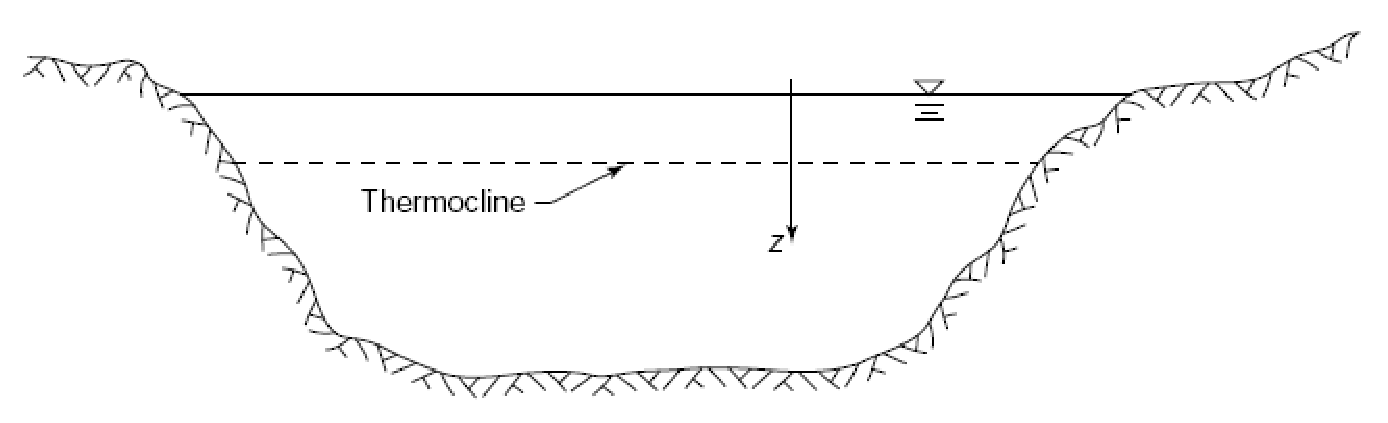
\includegraphics[height=3.5cm]{./images/alpine_lake.eps}}
\caption{Schematic of a stratified alpine lake.}
\label{fig:alpine-lake}
\end{figure}


However,
\textcolor{red}{what we need is the equation that predict the
  time-evolution of concentration $C(t)$ in space due to diffusive
  transport. Can we find it out? }

The mass change $\dot{m_x}$ across the area $A$ along the x-axis is
also the change in concentration, i.e. $A$ is a rectangle ($A=\delta
y\delta z$).
\begin{equation}
  \label{eq:176}
  \dot{m_x} = \int\int_A J_x\vec{n}dA = J_xA
\end{equation}
with $\vec{n}$ is the unit vector normal to the surface.  Extending to
three dimension, we examine a control volume (CV) of size $(\delta x,
\delta y, \delta z)$ as shown in Fig.~\ref{fig:diff-volume}. The
change in mass is given
\begin{equation}
  \label{eq:177}
  \frac{\partial M}{\partial t} = \sum \dot{m}_{in} - \sum
  \dot{m}_{out} = (\delta \dot{m_x}, \delta \dot{m_y}, \delta \dot{m_z})
\end{equation}

\begin{figure}[hbt]
 \centerline{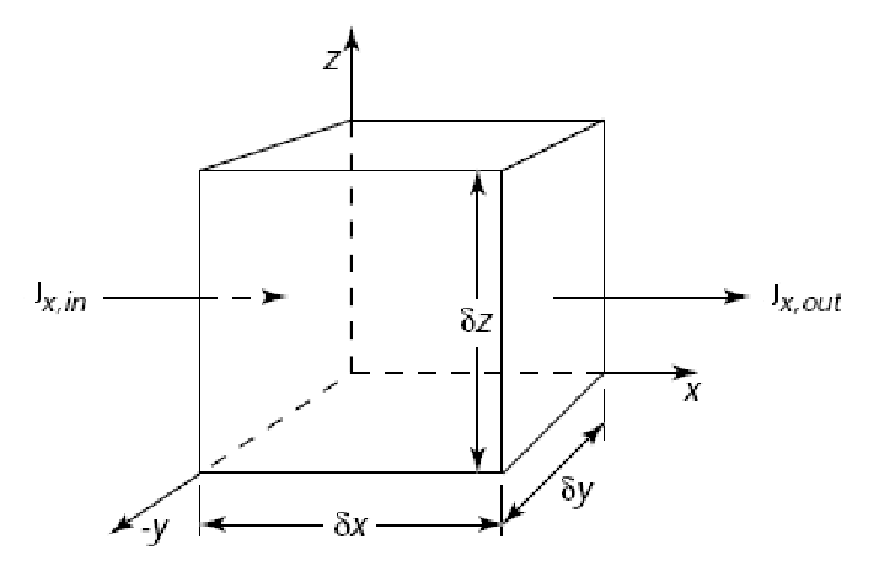
\includegraphics[height=5cm]{./images/diff-volume.eps}}
\caption{Differential control volume for derivation of the diffusion equation}
\label{fig:diff-volume}
\end{figure}

Using Fick's law, we have
\begin{equation}
  \label{eq:178}
  \begin{split}
    J_{x,in} &= -D\frac{\partial C}{\partial x}|_1\\
    J_{x,out} &= -D\frac{\partial C}{\partial x}|_2
  \end{split}
\end{equation}
Then, the net flux in the $x$-direction is
\begin{equation}
  \label{eq:180}
  \delta \dot{m}_x = - D\delta y \delta z \left( \frac{\partial
      C}{\partial x}|_1 - \frac{\partial C}{\partial x}|_2 \right)
\end{equation}

To estimate $ \frac{\partial C}{\partial x}|_2$ from $
\frac{\partial C}{\partial x}|_1$, the powerful technique first-order
Taylor series is utilized.
\begin{equation}
  \label{eq:181}
   \frac{\partial C}{\partial x}|_2 =  \frac{\partial C}{\partial
     x}|_1 + \frac{\partial}{\partial x}(\frac{\partial C}{\partial
     x}|_1)\delta x + R(2)
\end{equation}
with $R(2)$ is higher order terms and can be ignored. Then
\begin{equation}
  \label{eq:182}
  \delta \dot{m}_x =  D\delta y \delta z \frac{\partial
    C^2}{\partial^2 x} \delta x 
\end{equation}

Similarly, the formula for the net flux in $y$- and $z$- directions
\begin{equation}
  \label{eq:183}
  \begin{split}
    \delta \dot{m}_y &= D \delta x \delta y \delta z \frac{\partial
    C^2}{\partial^2 y}  \\
    \delta \dot{m}_z &= D \delta x \delta y \delta z \frac{\partial
    C^2}{\partial^2 z}  
  \end{split}
\end{equation}

As the mass $m$ is related to the concentration, i.e. $m=C\times
V=C\delta x\delta y\delta z$. Thus, $\dot{m} = \frac{\delta
  C}{\delta
  t}
\delta x \delta y \delta z$. Combine all equations together, finally
\begin{equation}
  \label{eq:184}
  \frac{\partial C}{\delta t} = D(\frac{\partial C^2}{\partial^2x} +
  \frac{\partial C^2}{\partial^2y} + \frac{\partial C^2}{\partial^2z}
  ) = D\nabla^2 C
%  = D\frac{\partial C^2}{\partial x_i^2}
\end{equation}
which is called {\bf Fick's second law}.  The previous question is now
answered.
\textcolor{red}{This is the fundamental equation in environmental
  fluid mechanics.}
Yet, another question arises: \textcolor{red}{can we solve it?} -
There are different ways, and one of them is Fischer method or the
so-called {\bf similarity method}.  The power of a similarity method
is that it turns a partial differential equation (PDE) into an
ordinary differential equation (ODE), which is the goal of any
solution method for PDEs.

{\bf Example}: Using similarity method to solve the one-dimensional
diffusion problem in a narrow pipe (radius $a$, infinite length). At
time $t=0$, a mass of tracer $M$ is injected uniformly across the
cross-section of area $A=\pi a^2$ at point $x=0$. We need to find the
equation for the concentration (the spread) of the tracer in the
$x$-direction over time due to molecular diffusion alone: $C_x(t)$.

\begin{itemize}
\item Under the assumption, i.e. $\partial C/\partial y = \partial
  C/\partial z = 0$, the equation we need to solve is
  \begin{equation}
    \label{eq:187}
    \frac{\partial C}{\partial t} = D\frac{\partial C^2}{\partial^2 x}
  \end{equation}

\item No particle can travel to infinity, $C_{\pm\infty}(t)=0$.

\item To specify the initial condition (only at $x=0$ has the
  particles with uniform distribution $M/A$, other locations $x \ne
  0$, the concentration is zero), the {\it Direct delta function} $\delta x$
  is used
  \begin{equation}
    \label{eq:188}
    C_x(0) = (M/A) \delta x
  \end{equation}

\item Mathematically, the total inject mass is
  \begin{equation}
    \label{eq:189}
    M = \int_V C_x(t)dV = \int_{-\infty}^\infty \int_0^a
    (M/A)\delta(x) 2\pi r dr dx
  \end{equation}
as $dV = 2\pi r drdx$.

\item Dimensional analysis technique is utilized: first, we need to
  identify all variables and noting their units (dependent: $C$
  (M/L$^3$), independent: $M/A$ [M/L$^2$], $D$ [L$^2$/T], x [L], $t$
  [T]) with M(ass), L(ength), T(ime). There are $m=5$ parameters and
  $n=3$ different dimensions. Then, we can form two dimensionless
  variables
  \begin{equation}
    \label{eq:191}
    \begin{split}
      \pi_1 &= \frac{C}{M/(A\sqrt{Dt})} \\
      \pi_2 &= \frac{x}{\sqrt{Dt}}
    \end{split}
  \end{equation}
  {\bf TIPS}: There are different arrangements to create $\pi_1, \pi_2$,
  however the rule of thumb is:
  (1) make sure the dependent variable can be obtained from $\pi_1$
  conveniently, (2) $\pi_1 = f(\pi_2)$, then
\begin{equation}
  \label{eq:192}
  C_x(t) = \frac{M}{A\sqrt{Dt}} f(\pi_2) = \frac{M}{A\sqrt{Dt}} f(\frac{x}{\sqrt{Dt}})
\end{equation}
with $f(.)$ is an unknown function known as
{\bf a similarity solution} because $C_x(t)$ has the same shape in
$x$-direction at all time $t$. The next question is
\textcolor{red}{what is the shape of $C$?}.

The detail how to solve the solution analytically is
skipped\footnote{since numerical methods are commonly used in
  practical problems},
let's just look at the actual solution (analytical solution) to see
how powerful the dimensional analysis gives us.
\begin{equation}
  \label{eq:193}
  C =  \frac{M}{A\sqrt{4\pi Dt}} \exp(\frac{-x^2}{4Dt})
\end{equation}
\textcolor{red}{How can we find this solution?} - There are two
primary ways: (1) plot the experimental data and then predict the form
of the smooth curve fitting the plot, then use some curve fitting tool
to estimate the parameter with the coordinate $(\pi_1, \pi_2)$, (2)
using eq.~\eqref{eq:192} as the solution for the differential equation
and solve it analytically with initial and boundary conditions
provided above [NOTE: For information on software for curve fitting, read
'Data Visualization' book].
The solution in 3D motion is
\begin{equation}
  \label{eq:194}
  C(x,y,z,t) = \frac{M}{4\pi t\sqrt{4\pi D_x D_y D_z}}
  \exp(-\frac{x^2}{4D_x t} -\frac{y^2}{4D_y t} -  \frac{z^2}{4D_z t})
\end{equation}

\item The maximum concentration is when the first-order derivative is
  zero and this can be achieved when the exponential part is zero or
  $x=y=z=0$.

\item Interpretation of the similarity solution: The shape of the
  concentration is bell-shaped, or its distribution is a Gaussian
  distribution with variance $\sigma^2 = 2Dt$. 

\item Regardless of the time, the values of mass $M$, concentration
  $D$ and the ratio $C/C_{mas}$ are always constant. 
\end{itemize}


\subsubsection{Turbulent diffusion}
\label{sec:turbulent-diffusion}

Turbulence also causes a kind of random, chaotic motion that behaves
asymptotically like Fickian diffusion. However, the Fickian diffusion
is a random yet smooth motion, while the turbulent motion is purely
random,
disorder\footnote{the chaotic is observed at the macroscopic level,
  yet at the microscopic level, it is highly organized}.
In essence, turbulent motion is much larger than molecular motion, and
turbulent diffusion coefficients $D_t$ are much larger than molecular
diffusion coefficients $D_m$.

Since turbulent diffusion obeys the same Fickian flux law, then the
turbulent diffusive flux $J_{z,t}$ can be related to the molecular
diffusive flux $J_{z,t} = J_z$ by the equation
\begin{equation}
  \label{eq:186}  
  J_{z,t} = J_{z,m} \frac{D_t}{D_m}
\end{equation}
\subsection{Advection Diffusion}
\label{sec:advection}

In the previous example, without the flow of the pipe fluid, the
injected tracer spread equally in all direction whose concentration
following Gaussian distribution with the center of the mass is at the
initial location $(0,0,0)$. Now, if we open the valve and allow water
to flow in the pipe, we expect the center of the mass to move with the
mean flow velocity in the pipe. It means that the central is now
\begin{equation}
  \label{eq:195}
  \eta = x - (x_0 + ut)
\end{equation}
with $\eta$ is the moving reference frame, $x_0$ is the injection
point of the tracer (zero in the previous example), $u$ is the mean
flow velocity and $ut$ is the distance traveled by the center of the
mass in time $t$. This is the mechanism of advection.

Advection is a transport mechanism of a substance by a moving
fluid. Advection is a conserved property of a moving fluid and is
described mathematically as a {\it vector field}. So, we expect that
the equation for advection diffusion to be something like this
\begin{equation}
  \label{eq:196}
   C =  \frac{M}{A\sqrt{4\pi Dt}} \exp
   \left(\frac{-(x-(x_0+ut))^2}{4Dt} \right)
\end{equation}
We need test this prediction by deriving the equation for advection
diffusion equation. This relies on the
{\it principle of superposition}: advection and diffusion can be added
together if they are linearly independent. However, how do we know
they are independent processes? Two processes are dependent only one
process feeds back on the other. Diffusion is a random process, with
random step $\pm \delta x$. With advection, each molecule will move
$u\delta t$ in the cross-flow direction. So, the advection just add
something to that random step in diffusion. The net movement under
advection-diffusion is $u\delta t \pm \delta t$. Thus, the total flux
in the $x$-direction is
\begin{equation}
  \label{eq:197}
  J_x = uC + J_{x,Fickian} = uC - D \frac{\partial C}{\partial x}
\end{equation}
with $J_{x,Fickian}$ is the Fickian flux described in the previous
section.

Here, $uC$ is the correct term for advection.  Use the flux law and
the conservation of mass... finally, we have
\begin{equation}
  \label{eq:198}
  \frac{\partial C}{\partial t} + \nabla \dot (uC) = D\nabla^2 C
\end{equation}
 or in Einstein notation
 \begin{equation}
   \label{eq:199}
   \frac{\partial C}{\partial t} + \frac{\partial u_iC}{\partial x_i}
   = D\frac{\partial C^2}{\partial x_i^2}
 \end{equation}
which is the {\bf advection-diffusion equation} with the right
hand-side is
\begin{equation}
  \label{eq:200}
  \frac{\partial}{\partial x_i} \left( D_{ij} \frac{\partial
      C}{\partial x_j} \right)
\end{equation}

\subsection{Convection}
\label{sec:convection}

Many people use the term convection synonymously with
advection. However, convection describes the transport by combined
molecular and eddy diffusion, while advection refers to transport with
a general flow of fluid.


\section{Chemical Reaction}
\label{sec:chemical-reaction}

Just a remind, the equation that represents the change in density
$C(x,t)$ with time when it is sufficiently smooth
\begin{equation}
  \label{eq:217}
  \frac{dC(\mathbf{x},t)}{dt} = D\nabla^2C(\mathbf{x},t)
\end{equation}
with $\mathbf{x}$ is the 3D coordinate of the particle. 

Now, what if we want to write a differential equation describing the
time dependence of the density in terms of various spatial
derivatives, i.e. $\frac{d}{dx}C(x,t), \frac{d}{dxdy}C(x,t),
\frac{d}{dx^2}C(x,t), ...$.


A system of reacting and diffusing molecules are called
reaction-diffusion systems. Chemical reactions causes the molecular
densities to change with time even there is no diffusion. The general
dynamic of the system using a set of coupled equations of the form
\begin{equation}
  \label{eq:218}
  \frac{dC_i(\mathbf{x},t)}{dt} = D\nabla^2C_i(\mathbf{x},t)+R_i(\{n_j(\mathbf{x},t)\})
\end{equation}
where $R_i(\{n_j(\mathbf{x},t)\})$ is the rate of changes in the
concentration of a molecular species $i$.


Assumptions:
\begin{enumerate}
\item the density is not too rapidly varying in space, so that local
  reaction rate depends only on the local densities and not their
  gradients

\item diffusion time between reactions is large compared to the time
  of reaction.

\item 
\end{enumerate}

\section{Incorporating transformation with advective-diffusion equation}
\label{sec:incorp-transf-with}

\subsection{Advective-reacting diffusion equation}
\label{sec:advect-react-diff}


\subsection{Reaction-diffusion equation}
\label{sec:react-diff-equat}

A system of chemical substances - morphogens - diffusing through a
mass of tissue of a given geometrical form and reacting together
within it, is adequate to describe for the main phenomena of
morphogenesis - the biological processes of forming
patterns/structures. What laws to control the development in such
situations?
\begin{itemize}
\item The diffusion follows the ordinary law of diffusion, i.e. moving
  from regions of high concentration to those of lower concentration,
  at a rate proportional to the gradient of concentration and also the
  ``diffusibility'' of the substance. If there is no cell walls, the
  reaction would inversely proportional to the square root of the
  molecular weights.
\item The reaction rate is assumed to obey the ``law of mass
  action'', i.e. the reaction rate is proportional to the
  concentrations, i.e the chance of encountering of the molecules. 
\end{itemize}

There are in fact 6 different forms :
\begin{enumerate}
\item stationary waves on the isolated ring of cells, account for the
  phenomena of phyllotaxis.
\item tentacle patterns on Hydra and for whorled leaves. 
\item gastrulation on a sphere 
\item pattern reminiscent of dappling 
\end{enumerate}


The first person to describe this phenomena is
Turing\cite{turing1952cbm}\footnote{\url{http://www.turingarchive.org/viewer/?id=476&title=2}}.
Turing studies the morphogenesis of the embryo. A solution of linear
differential equations with constant coefficients is in the form of a
sum $\sum A e^{bt}$ with $A, b$ are complex quantities. The real part
should be
\begin{equation}
  \label{eq:219}
  Real(Ae^{bt})=A'e^{\alpha t} \cos(\beta t + \phi)
\end{equation}
with $A=A'ei^\phi, b=\alpha+i\beta$.

\begin{enumerate}
\item $\alpha=0$: sinusoidal oscillation
\item $\alpha<0$: a damped oscillation
\item $\alpha>0$: an oscillation of ever-increasing amplitude.
  \begin{equation}
    \label{eq:220}
    \frac{dy}{dt} = \alpha y; \; \alpha > 0
  \end{equation}
\end{enumerate}
At a sufficient great lapse of time, all the terms $Ae^{bt}$ will
become negligible in comparison with the terms which has the greatest
real part. Unless this greatest real part is zero, these dominant
terms will eventually either tend to zero (for negative real part) or
to infinite values (for positive real part).

\begin{enumerate}
\item any of the numbers $b$ has a positive real part ($\alpha_i>0$),
  the system is unstable
\item 
\end{enumerate}


Suppose that there are $N$ cells and $M$ types of morphogens. Then, at
a specific time point, there will be a number of a type of morphogen
in a given cell. Thus, to know the state of a single cell, we need M
values. Accordingly, to know the state of a system with $N$ cells, we
need $MN$ number of values. These number changes with time, partly
because of reactions, partly because of diffusion.

\begin{itemize}
\item To know the value of a given morphogen in a given cell due to
  diffusion, we need to know the concentration of that morphogen
  (i.e. the number of molecules of that type of morphogen) in the cell
  and in all neighboring cells, as well as the rate of diffusion for
  that morphogen
\item TO know the value of a given morphogen in a given cell due to
  reaction, we need to know the concentration of all types of
  morphogens in that cell only. 
\end{itemize}


%%% Local Variables: 
%%% mode: latex
%%% TeX-master: "thermo-stat"
%%% End: 
